\documentclass{article}
\usepackage{amsmath}
\usepackage{color,pxfonts,fix-cm}
\usepackage{latexsym}
\usepackage[mathletters]{ucs}
\DeclareUnicodeCharacter{8211}{\textendash}
\DeclareUnicodeCharacter{46}{\textperiodcentered}
\DeclareUnicodeCharacter{58}{$\colon$}
\DeclareUnicodeCharacter{8226}{$\bullet$}
\DeclareUnicodeCharacter{191}{\textquestiondown}
\DeclareUnicodeCharacter{62}{\textgreater}
\usepackage[T1]{fontenc}
\usepackage[utf8x]{inputenc}
\usepackage{pict2e}
\usepackage{wasysym}
\usepackage[english]{babel}
\usepackage{tikz}
\pagestyle{empty}
\usepackage[margin=0in,paperwidth=612pt,paperheight=792pt]{geometry}
\begin{document}
\definecolor{color_29791}{rgb}{0,0,0}
\begin{tikzpicture}[overlay]\path(0pt,0pt);\end{tikzpicture}
\begin{picture}(-5,0)(2.5,0)
\put(57,-34.90198){\fontsize{11.9552}{1}\usefont{T1}{cmr}{b}{n}\selectfont\color{color_29791}CSE 406-Project Report The Hive}
\end{picture}
\begin{tikzpicture}[overlay]
\path(0pt,0pt);
\draw[color_29791,line width=0.996pt]
(57pt, -39.58398pt) -- (525pt, -39.58398pt)
;
\end{tikzpicture}
\begin{picture}(-5,0)(2.5,0)
\put(228,-218.879){
\includegraphics[width=126pt,height=126pt]{latexImage_ff260eee2f38ae1b9dbcc8b793d04540.png}}
\put(132.775,-312.797){\fontsize{17.2154}{1}\usefont{T1}{cmr}{b}{n}\selectfont\color{color_29791}CSE406-Computer Security Sessional}
\put(59.54399,-334.714){\fontsize{17.2154}{1}\usefont{T1}{cmr}{b}{n}\selectfont\color{color_29791}Report on TheHive - an open source and free Security}
\put(172.716,-356.632){\fontsize{17.2154}{1}\usefont{T1}{cmr}{b}{n}\selectfont\color{color_29791}Incident Response Platform}
\put(215.228,-391.501){\fontsize{11.9552}{1}\usefont{T1}{cmr}{m}{n}\selectfont\color{color_29791} 1905102: Shafiul Haque}
\put(215.228,-419.397){\fontsize{11.9552}{1}\usefont{T1}{cmr}{m}{n}\selectfont\color{color_29791}1905116: Md. Sayeeduzzaman}
% \begin{center}
%     \Huge % Adjust font size as needed
%     Your Text Here
% \end{center}
\put(160.285,-497.24){\fontsize{11.9552}{1}\usefont{T1}{cmr}{m}{n}\selectfont\color{color_29791}Department of Computer Science and Engineering,}
\put(157.458,-511.188){\fontsize{11.9552}{1}\usefont{T1}{cmr}{m}{n}\selectfont\color{color_29791}Bangladesh University of Engineering \& Technology}
\put(240.924,-540.611){\fontsize{11.9552}{1}\usefont{T1}{cmr}{m}{n}\selectfont\color{color_29791}March 9, 20}
\end{picture}

\newpage
\begin{tikzpicture}[overlay]\path(0pt,0pt);\end{tikzpicture}
\begin{picture}(-5,0)(2.5,0)
\put(57,-34.90198){\fontsize{11.9552}{1}\usefont{T1}{cmr}{b}{n}\selectfont\color{color_29791}CSE 406-Project Report TheHive}
\end{picture}
\begin{tikzpicture}[overlay]
\path(0pt,0pt);
\draw[color_29791,line width=0.996pt]
(57pt, -39.58398pt) -- (525pt, -39.58398pt)
;
\end{tikzpicture}
\begin{picture}(-5,0)(2.5,0)
\put(57,-71.96301){\fontsize{14.3462}{1}\usefont{T1}{cmr}{b}{n}\selectfont\color{color_29791}Contents}
\put(57,-93.88){\fontsize{9.9626}{1}\usefont{T1}{cmr}{b}{n}\selectfont\color{color_29791}1 Introduction 3}
\put(56.99997,-115.798){\fontsize{9.9626}{1}\usefont{T1}{cmr}{b}{n}\selectfont\color{color_29791}2 Overview of the Source Code 3}
\put(71.94397,-127.753){\fontsize{9.9626}{1}\usefont{T1}{cmr}{m}{n}\selectfont\color{color_29791}2.1}
\put(503.9301,-127.753){\fontsize{9.9626}{1}\usefont{T1}{cmr}{m}{n}\selectfont\color{color_29791}}
\put(520.0197,-127.753){\fontsize{9.9626}{1}\usefont{T1}{cmr}{m}{n}\selectfont\color{color_29791}4}
\put(71.94397,-139.709){\fontsize{9.9626}{1}\usefont{T1}{cmr}{m}{n}\selectfont\color{color_29791}2.2}
\put(503.9291,-139.709){\fontsize{9.9626}{1}\usefont{T1}{cmr}{m}{n}\selectfont\color{color_29791}}
\put(520.0187,-139.709){\fontsize{9.9626}{1}\usefont{T1}{cmr}{m}{n}\selectfont\color{color_29791}4}
\put(71.94397,-151.664){\fontsize{9.9626}{1}\usefont{T1}{cmr}{m}{n}\selectfont\color{color_29791}2.3}
\put(503.9261,-151.664){\fontsize{9.9626}{1}\usefont{T1}{cmr}{m}{n}\selectfont\color{color_29791}}
\put(520.0157,-151.664){\fontsize{9.9626}{1}\usefont{T1}{cmr}{m}{n}\selectfont\color{color_29791}4}
\put(71.94397,-163.619){\fontsize{9.9626}{1}\usefont{T1}{cmr}{m}{n}\selectfont\color{color_29791}2.4}
\put(503.9241,-163.619){\fontsize{9.9626}{1}\usefont{T1}{cmr}{m}{n}\selectfont\color{color_29791}}
\put(520.0137,-163.619){\fontsize{9.9626}{1}\usefont{T1}{cmr}{m}{n}\selectfont\color{color_29791}4}
\put(71.94397,-175.574){\fontsize{9.9626}{1}\usefont{T1}{cmr}{m}{n}\selectfont\color{color_29791}2.5}
\put(503.9331,-175.574){\fontsize{9.9626}{1}\usefont{T1}{cmr}{m}{n}\selectfont\color{color_29791}}
\put(520.0227,-175.574){\fontsize{9.9626}{1}\usefont{T1}{cmr}{m}{n}\selectfont\color{color_29791}4}
\put(71.94397,-187.5291){\fontsize{9.9626}{1}\usefont{T1}{cmr}{m}{n}\selectfont\color{color_29791}2.6}
\put(503.9281,-187.5291){\fontsize{9.9626}{1}\usefont{T1}{cmr}{m}{n}\selectfont\color{color_29791}}
\put(520.0177,-187.5291){\fontsize{9.9626}{1}\usefont{T1}{cmr}{m}{n}\selectfont\color{color_29791}5}
\put(71.94397,-199.485){\fontsize{9.9626}{1}\usefont{T1}{cmr}{m}{n}\selectfont\color{color_29791}2.7}
\put(503.9301,-199.485){\fontsize{9.9626}{1}\usefont{T1}{cmr}{m}{n}\selectfont\color{color_29791}}
\put(520.0197,-199.485){\fontsize{9.9626}{1}\usefont{T1}{cmr}{m}{n}\selectfont\color{color_29791}5}
\put(71.94397,-211.4401){\fontsize{9.9626}{1}\usefont{T1}{cmr}{m}{n}\selectfont\color{color_29791}2.8}
\put(503.9271,-211.4401){\fontsize{9.9626}{1}\usefont{T1}{cmr}{m}{n}\selectfont\color{color_29791}}
\put(520.0167,-211.4401){\fontsize{9.9626}{1}\usefont{T1}{cmr}{m}{n}\selectfont\color{color_29791}5}
\put(71.94397,-223.3951){\fontsize{9.9626}{1}\usefont{T1}{cmr}{m}{n}\selectfont\color{color_29791}2.9}
\put(503.9312,-223.3951){\fontsize{9.9626}{1}\usefont{T1}{cmr}{m}{n}\selectfont\color{color_29791}}
\put(520.0208,-223.3951){\fontsize{9.9626}{1}\usefont{T1}{cmr}{m}{n}\selectfont\color{color_29791}5}
\put(71.94397,-235.3501){\fontsize{9.9626}{1}\usefont{T1}{cmr}{m}{n}\selectfont\color{color_29791}2.10}
\put(503.9282,-235.3501){\fontsize{9.9626}{1}\usefont{T1}{cmr}{m}{n}\selectfont\color{color_29791}}
\put(520.0178,-235.3501){\fontsize{9.9626}{1}\usefont{T1}{cmr}{m}{n}\selectfont\color{color_29791}5}
\put(71.94397,-247.3051){\fontsize{9.9626}{1}\usefont{T1}{cmr}{m}{n}\selectfont\color{color_29791}2.11}
\put(503.9241,-247.3051){\fontsize{9.9626}{1}\usefont{T1}{cmr}{m}{n}\selectfont\color{color_29791}}
\put(520.0137,-247.3051){\fontsize{9.9626}{1}\usefont{T1}{cmr}{m}{n}\selectfont\color{color_29791}5}
\put(56.99997,-269.2231){\fontsize{9.9626}{1}\usefont{T1}{cmr}{b}{n}\selectfont\color{color_29791}3 Key Features }
\put(56.99997,-291.1411){\fontsize{9.9626}{1}\usefont{T1}{cmr}{b}{n}\selectfont\color{color_29791}4 Key Components }
\put(71.94397,-303.0961){\fontsize{9.9626}{1}\usefont{T1}{cmr}{m}{n}\selectfont\color{color_29791}4.1}
\put(503.9301,-303.0961){\fontsize{9.9626}{1}\usefont{T1}{cmr}{m}{n}\selectfont\color{color_29791}}
\put(520.0197,-303.0961){\fontsize{9.9626}{1}\usefont{T1}{cmr}{m}{n}\selectfont\color{color_29791}6}
\put(71.94397,-315.0511){\fontsize{9.9626}{1}\usefont{T1}{cmr}{m}{n}\selectfont\color{color_29791}4.2}
\put(503.9261,-315.0511){\fontsize{9.9626}{1}\usefont{T1}{cmr}{m}{n}\selectfont\color{color_29791}}
\put(520.0157,-315.0511){\fontsize{9.9626}{1}\usefont{T1}{cmr}{m}{n}\selectfont\color{color_29791}6}
\put(71.94397,-327.0061){\fontsize{9.9626}{1}\usefont{T1}{cmr}{m}{n}\selectfont\color{color_29791}4.3}
\put(503.9241,-327.0061){\fontsize{9.9626}{1}\usefont{T1}{cmr}{m}{n}\selectfont\color{color_29791}}
\put(520.0137,-327.0061){\fontsize{9.9626}{1}\usefont{T1}{cmr}{m}{n}\selectfont\color{color_29791}6}
\put(71.94397,-338.9621){\fontsize{9.9626}{1}\usefont{T1}{cmr}{m}{n}\selectfont\color{color_29791}4.4}
\put(503.9271,-338.9621){\fontsize{9.9626}{1}\usefont{T1}{cmr}{m}{n}\selectfont\color{color_29791}}
\put(520.0167,-338.9621){\fontsize{9.9626}{1}\usefont{T1}{cmr}{m}{n}\selectfont\color{color_29791}6}
\put(56.99997,-360.8791){\fontsize{9.9626}{1}\usefont{T1}{cmr}{b}{n}\selectfont\color{color_29791}5 Documentation of Key features 6}
\put(71.94397,-372.8351){\fontsize{9.9626}{1}\usefont{T1}{cmr}{m}{n}\selectfont\color{color_29791}5.1}
\put(503.9271,-372.8351){\fontsize{9.9626}{1}\usefont{T1}{cmr}{m}{n}\selectfont\color{color_29791}}
\put(520.0167,-372.8351){\fontsize{9.9626}{1}\usefont{T1}{cmr}{m}{n}\selectfont\color{color_29791}6}
\put(94.85797,-384.7901){\fontsize{9.9626}{1}\usefont{T1}{cmr}{m}{n}\selectfont\color{color_29791}5.1.1}
\put(503.9321,-384.7901){\fontsize{9.9626}{1}\usefont{T1}{cmr}{m}{n}\selectfont\color{color_29791}}
\put(520.0217,-384.7901){\fontsize{9.9626}{1}\usefont{T1}{cmr}{m}{n}\selectfont\color{color_29791}6}
\put(94.85797,-396.7451){\fontsize{9.9626}{1}\usefont{T1}{cmr}{m}{n}\selectfont\color{color_29791}5.1.2}
\put(503.9321,-396.7451){\fontsize{9.9626}{1}\usefont{T1}{cmr}{m}{n}\selectfont\color{color_29791}}
\put(515.0404,-396.7451){\fontsize{9.9626}{1}\usefont{T1}{cmr}{m}{n}\selectfont\color{color_29791}10}
\put(94.85797,-408.7){\fontsize{9.9626}{1}\usefont{T1}{cmr}{m}{n}\selectfont\color{color_29791}5.1.3}
\put(503.9321,-408.7){\fontsize{9.9626}{1}\usefont{T1}{cmr}{m}{n}\selectfont\color{color_29791}}
\put(515.0404,-408.7){\fontsize{9.9626}{1}\usefont{T1}{cmr}{m}{n}\selectfont\color{color_29791}14}
\put(71.94397,-420.655){\fontsize{9.9626}{1}\usefont{T1}{cmr}{m}{n}\selectfont\color{color_29791}5.2}
\put(503.9291,-420.655){\fontsize{9.9626}{1}\usefont{T1}{cmr}{m}{n}\selectfont\color{color_29791}}
\put(515.0374,-420.655){\fontsize{9.9626}{1}\usefont{T1}{cmr}{m}{n}\selectfont\color{color_29791}15}
\put(94.85797,-432.61){\fontsize{9.9626}{1}\usefont{T1}{cmr}{m}{n}\selectfont\color{color_29791}5.2.1}
\put(503.9321,-432.61){\fontsize{9.9626}{1}\usefont{T1}{cmr}{m}{n}\selectfont\color{color_29791}}
\put(515.0404,-432.61){\fontsize{9.9626}{1}\usefont{T1}{cmr}{m}{n}\selectfont\color{color_29791}15}
\put(94.85797,-444.566){\fontsize{9.9626}{1}\usefont{T1}{cmr}{m}{n}\selectfont\color{color_29791}5.2.2}
\put(503.9261,-444.566){\fontsize{9.9626}{1}\usefont{T1}{cmr}{m}{n}\selectfont\color{color_29791}}
\put(515.0344,-444.566){\fontsize{9.9626}{1}\usefont{T1}{cmr}{m}{n}\selectfont\color{color_29791}24}
\put(71.94397,-456.521){\fontsize{9.9626}{1}\usefont{T1}{cmr}{m}{n}\selectfont\color{color_29791}5.3}
\put(503.9271,-456.521){\fontsize{9.9626}{1}\usefont{T1}{cmr}{m}{n}\selectfont\color{color_29791}}
\put(515.0354,-456.521){\fontsize{9.9626}{1}\usefont{T1}{cmr}{m}{n}\selectfont\color{color_29791}29}
\put(94.85797,-468.476){\fontsize{9.9626}{1}\usefont{T1}{cmr}{m}{n}\selectfont\color{color_29791}5.3.1}
\put(503.933,-468.476){\fontsize{9.9626}{1}\usefont{T1}{cmr}{m}{n}\selectfont\color{color_29791}}
\put(515.0413,-468.476){\fontsize{9.9626}{1}\usefont{T1}{cmr}{m}{n}\selectfont\color{color_29791}29}
\put(94.85797,-480.431){\fontsize{9.9626}{1}\usefont{T1}{cmr}{m}{n}\selectfont\color{color_29791}5.3.2}
\put(503.9301,-480.431){\fontsize{9.9626}{1}\usefont{T1}{cmr}{m}{n}\selectfont\color{color_29791}}
\put(515.0384,-480.431){\fontsize{9.9626}{1}\usefont{T1}{cmr}{m}{n}\selectfont\color{color_29791}30}
\end{picture}
\begin{tikzpicture}[overlay]
\path(0pt,0pt);
\draw[color_29791,line width=0.996pt]
(57pt, -727.435pt) -- (525pt, -727.435pt)
;
\end{tikzpicture}
\begin{picture}(-5,0)(2.5,0)
\put(519.521,-739.888){\fontsize{9.9626}{1}\usefont{T1}{cmr}{b}{n}\selectfont\color{color_29791}2}
\end{picture}
\newpage
\begin{tikzpicture}[overlay]\path(0pt,0pt);\end{tikzpicture}


\begin{picture}(-5,0)(2.5,0)
\put(57,-71.96301){\fontsize{14.3462}{1}\usefont{T1}{cmr}{b}{n}\selectfont\color{color_29791}1 Introduction}
\put(57,-93.784){\fontsize{9.9626}{1}\usefont{T1}{cmr}{m}{n}\selectfont\color{color_29791}TheHive is an open source and free securit y incident response platform that helps security professionals}
\put(57,-105.739){\fontsize{9.9626}{1}\usefont{T1}{cmr}{m}{n}\selectfont\color{color_29791}deal with cyber threats and incidents. It is developed and maintained by TheHive Project, a community of}
\put(57,-117.694){\fontsize{9.9626}{1}\usefont{T1}{cmr}{m}{n}\selectfont\color{color_29791}security experts and enthusiasts. The source code of TheHive is hosted on GitHub, where any one can access,}
\put(57,-129.649){\fontsize{9.9626}{1}\usefont{T1}{cmr}{m}{n}\selectfont\color{color_29791}review, or contribute to it. In this rep ort, we will provide a high level overview of the main modules.}

\put(57,-277.177){
\includegraphics[width=468pt,height=121.68pt]{latexImage_0b219125a30ecc65413c02f31badaee1.png}}
\put(57,-326.118){\fontsize{14.3462}{1}\usefont{T1}{cmr}{b}{n}\selectfont\color{color_29791}2 Overview of the Source Code}
\put(57,-347.939){\fontsize{9.9626}{1}\usefont{T1}{cmr}{m}{n}\selectfont\color{color_29791}The source code of TheHive is written mainly in Scala, a general-purpose programming language that runs}
\put(57,-359.894){\fontsize{9.9626}{1}\usefont{T1}{cmr}{m}{n}\selectfont\color{color_29791}on the Java Virtual Machine (JVM). The code is organized in to several modules and packages , each with a}
\put(57,-371.85){\fontsize{9.9626}{1}\usefont{T1}{cmr}{m}{n}\selectfont\color{color_29791}specific purpose and functionality. Figure 1 shows the structure of the source code}
\put(57,-659.774){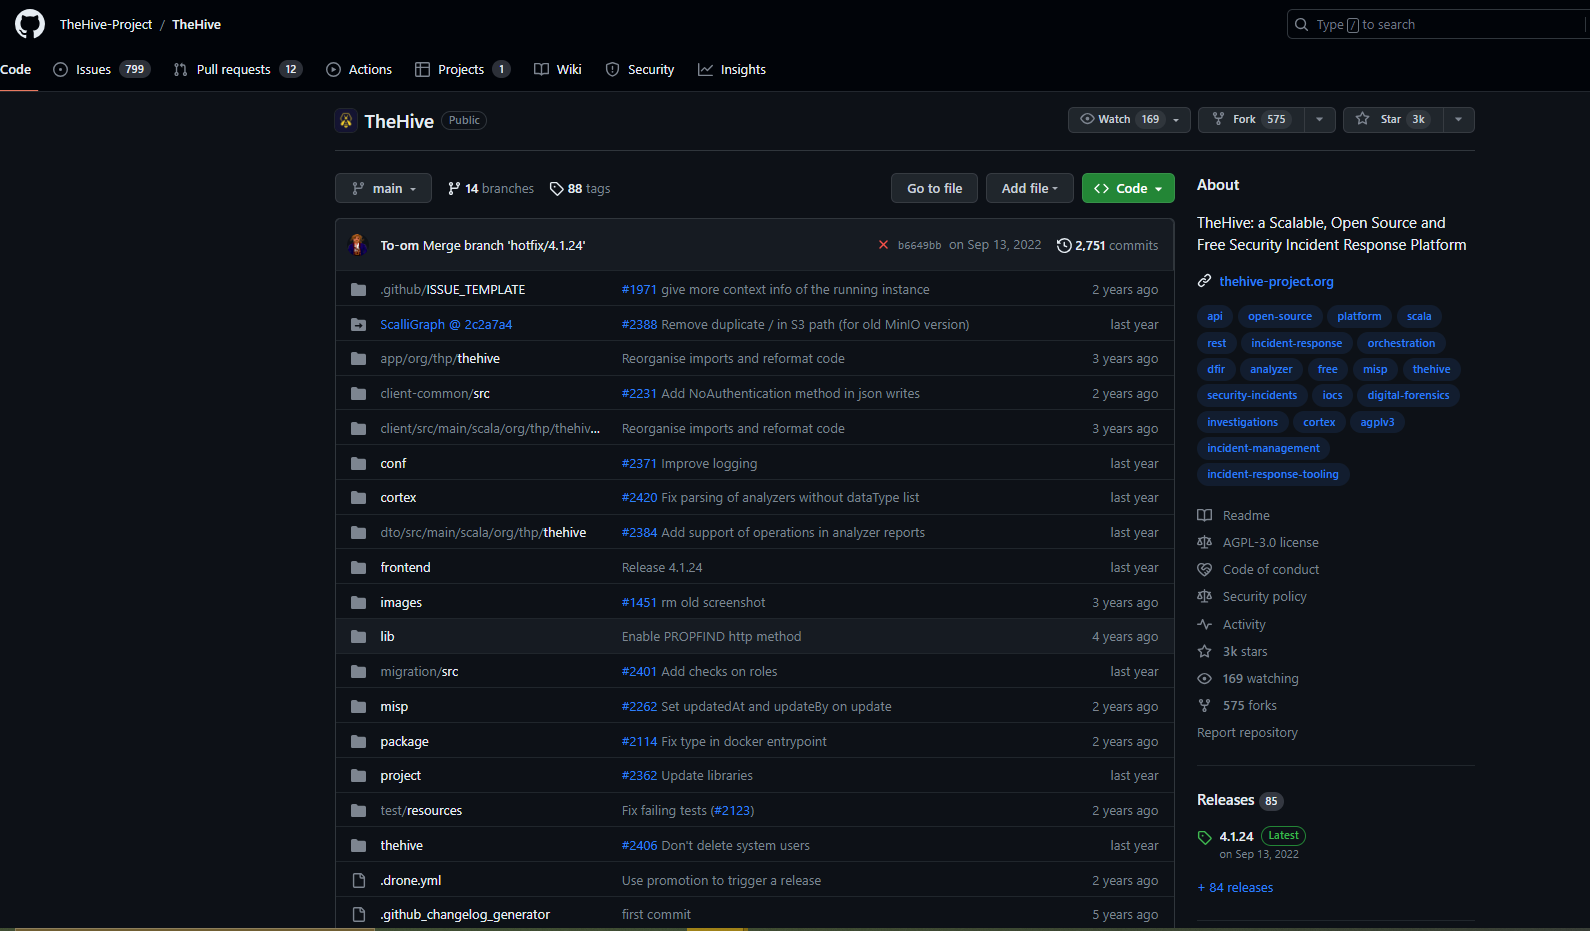
\includegraphics[width=468.0038pt,height=274.0324pt]{latexImage_c9be62a3df829223d0ad26cb1cc53dbd.png}}
\put(172.514,-678.105){\fontsize{9.9626}{1}\usefont{T1}{cmr}{m}{n}\selectfont\color{color_29791}Figure 1: The structure of the source code of TheHive}
\put(57.00001,-703.665){\fontsize{9.9626}{1}\usefont{T1}{cmr}{m}{n}\selectfont\color{color_29791}We will briefly describe the main modules and packages of the source code in the following subsections.}
\end{picture}
\begin{tikzpicture}[overlay]
\path(0pt,0pt);
\draw[color_29791,line width=0.996pt]
(57pt, -727.435pt) -- (525pt, -727.435pt)
;
\end{tikzpicture}
\begin{picture}(-5,0)(2.5,0)

\put(519.521,-739.888){\fontsize{9.9626}{1}\usefont{T1}{cmr}{b}{n}\selectfont\color{color_29791}3}
\end{picture}
\newpage
\begin{tikzpicture}[overlay]\path(0pt,0pt);\end{tikzpicture}

\begin{picture}(-5,0)(2.5,0)
\put(57,-71.96301){\fontsize{11.9552}{1}\usefont{T1}{cmr}{b}{n}\selectfont\color{color_29791}2.1 app}
\put(57,-90.35199){\fontsize{9.9626}{1}\usefont{T1}{cmr}{m}{n}\selectfont\color{color_29791}This module contains the core logic and functionality of TheHive. It includes the following packages:}
\put(71.945,-108.285){\fontsize{9.9626}{1}\usefont{T1}{cmr}{m}{n}\selectfont\color{color_29791}• org.thp.thehive : This package contains the main classes and traits that define the application, such}
\put(81.907,-120.24){\fontsize{9.9626}{1}\usefont{T1}{cmr}{m}{n}\selectfont\color{color_29791}as TheHive App , TheHive Module, and TheHive Config .}
\put(71.94501,-138.173){\fontsize{9.9626}{1}\usefont{T1}{cmr}{m}{n}\selectfont\color{color_29791}• org.thp.thehive.controllers : This package contains the controllers that handle the HTTP requests}
\put(81.90701,-150.128){\fontsize{9.9626}{1}\usefont{T1}{cmr}{m}{n}\selectfont\color{color_29791}and responses for the different endpoints of the application, such as Cases, Tasks, Observables, Alerts,}
\put(81.90701,-162.083){\fontsize{9.9626}{1}\usefont{T1}{cmr}{m}{n}\selectfont\color{color_29791}and Users.}
\put(71.94501,-180.016){\fontsize{9.9626}{1}\usefont{T1}{cmr}{m}{n}\selectfont\color{color_29791}• org.thp.thehive.models : This package contains the case classes and objects that represent the data}
\put(81.90701,-191.971){\fontsize{9.9626}{1}\usefont{T1}{cmr}{m}{n}\selectfont\color{color_29791}models of the application, such as Case, Task, Observable, Alert, User, and Organisation.}
\put(71.94501,-209.904){\fontsize{9.9626}{1}\usefont{T1}{cmr}{m}{n}\selectfont\color{color_29791}• org.thp.thehive.services : This package contains the services that provide the business logic and}
\put(81.90701,-221.859){\fontsize{9.9626}{1}\usefont{T1}{cmr}{m}{n}\selectfont\color{color_29791}op erations for the datamodels, such as CaseSrv, TaskSrv, ObservableSrv, AlertSrv, UserSrv, and}
\put(81.90701,-233.814){\fontsize{9.9626}{1}\usefont{T1}{cmr}{m}{n}\selectfont\color{color_29791}OrganisationSrv.}
\put(71.94501,-251.747){\fontsize{9.9626}{1}\usefont{T1}{cmr}{m}{n}\selectfont\color{color_29791}• org.thp.thehive.connector : This package contains the classes and traits that enable the integration}
\put(81.90701,-263.702){\fontsize{9.9626}{1}\usefont{T1}{cmr}{m}{n}\selectfont\color{color_29791}with external tools and platforms, such as MISP and Cortex.}
\put(57.00002,-291.59){\fontsize{11.9552}{1}\usefont{T1}{cmr}{b}{n}\selectfont\color{color_29791}2.2 client}
\put(57.00002,-309.98){\fontsize{9.9626}{1}\usefont{T1}{cmr}{m}{n}\selectfont\color{color_29791}This module con tains the co de for the web-based user interfac e of TheHive. It includes the following packages:}
\put(71.94501,-327.9131){\fontsize{9.9626}{1}\usefont{T1}{cmr}{m}{n}\selectfont\color{color_29791}• org.thp.thehive.client : This package contains the classes and objects that define the client-side}
\put(81.90701,-339.868){\fontsize{9.9626}{1}\usefont{T1}{cmr}{m}{n}\selectfont\color{color_29791}application, such as ClientApp and ClientConfig .}
\put(71.94501,-357.8){\fontsize{9.9626}{1}\usefont{T1}{cmr}{m}{n}\selectfont\color{color_29791}• org.thp.thehive.client.pages : This package contains the components that render the different}
\put(81.90701,-369.756){\fontsize{9.9626}{1}\usefont{T1}{cmr}{m}{n}\selectfont\color{color_29791}pages of the user interface, such as Dash boardPage, CasePage, TaskP age, ObservablePage, AlertPage,}
\put(81.90701,-381.711){\fontsize{9.9626}{1}\usefont{T1}{cmr}{m}{n}\selectfont\color{color_29791}and UserPage .}
\put(71.94501,-399.644){\fontsize{9.9626}{1}\usefont{T1}{cmr}{m}{n}\selectfont\color{color_29791}• org.thp.thehive.client.services : This package contains the services that provide the client-side}
\put(81.907,-411.599){\fontsize{9.9626}{1}\usefont{T1}{cmr}{m}{n}\selectfont\color{color_29791}logic and operations for the user interface, such as ApiService, Notification Service, UserService, and}
\put(81.907,-423.554){\fontsize{9.9626}{1}\usefont{T1}{cmr}{m}{n}\selectfont\color{color_29791}Organisation Service.}
\put(57,-451.442){\fontsize{11.9552}{1}\usefont{T1}{cmr}{b}{n}\selectfont\color{color_29791}2.3 conf}
\put(57,-469.832){\fontsize{9.9626}{1}\usefont{T1}{cmr}{m}{n}\selectfont\color{color_29791}This module contains the configuration files for the application, such as application.conf and logback.xml.}
\put(57,-497.72){\fontsize{11.9552}{1}\usefont{T1}{cmr}{b}{n}\selectfont\color{color_29791}2.4 cortex}
\put(57,-516.11){\fontsize{9.9626}{1}\usefont{T1}{cmr}{m}{n}\selectfont\color{color_29791}This module contains the code for the integration with Cortex. It includes the following packages:}
\put(71.945,-534.0421){\fontsize{9.9626}{1}\usefont{T1}{cmr}{m}{n}\selectfont\color{color_29791}• org.thp.cortex.client : This package contains the classes and objects that define the client-side}
\put(81.90699,-545.9971){\fontsize{9.9626}{1}\usefont{T1}{cmr}{m}{n}\selectfont\color{color_29791}communication with Cortex, such as CortexClient and CortexConfig .}
\put(71.94501,-563.9301){\fontsize{9.9626}{1}\usefont{T1}{cmr}{m}{n}\selectfont\color{color_29791}• org.thp.cortex.dto : This pack age contains the case classes and objects that represent the data}
\put(81.90701,-575.8851){\fontsize{9.9626}{1}\usefont{T1}{cmr}{m}{n}\selectfont\color{color_29791}models of Cortex, such as Analyzer, Job, Report, Responder, Action, Response.}
\put(57.00001,-603.774){\fontsize{11.9552}{1}\usefont{T1}{cmr}{b}{n}\selectfont\color{color_29791}2.5 dto}
\put(57.00001,-622.1631){\fontsize{9.9626}{1}\usefont{T1}{cmr}{m}{n}\selectfont\color{color_29791}This module contains the code for the data transfer objects (DTOs) that are used to exchange data between}
\put(57.00001,-634.118){\fontsize{9.9626}{1}\usefont{T1}{cmr}{m}{n}\selectfont\color{color_29791}different layers of the application. It includes the following package:}
\put(71.94501,-652.051){\fontsize{9.9626}{1}\usefont{T1}{cmr}{m}{n}\selectfont\color{color_29791}• org.thp.thehive.dto : This package contains the case classes and objects that represent the DTOs}
\put(81.90701,-664.006){\fontsize{9.9626}{1}\usefont{T1}{cmr}{m}{n}\selectfont\color{color_29791}of TheHive , such as CaseDTO, TaskDTO, ObservableDTO, AlertDTO, UserDTO.}
\end{picture}
\begin{tikzpicture}[overlay]
\path(0pt,0pt);
\draw[color_29791,line width=0.996pt]
(57pt, -727.435pt) -- (525pt, -727.435pt)
;
\end{tikzpicture}
\begin{picture}(-5,0)(2.5,0)
\put(519.521,-739.888){\fontsize{9.9626}{1}\usefont{T1}{cmr}{b}{n}\selectfont\color{color_29791}4}
\end{picture}
\newpage
\begin{tikzpicture}[overlay]\path(0pt,0pt);\end{tikzpicture}
\begin{picture}(-5,0)(2.5,0)
\end{picture}
\begin{tikzpicture}[overlay]
\path(0pt,0pt);
\draw[color_29791,line width=0.996pt]
(57pt, -39.58398pt) -- (525pt, -39.58398pt)
;
\end{tikzpicture}
\begin{picture}(-5,0)(2.5,0)
\put(57,-71.96301){\fontsize{11.9552}{1}\usefont{T1}{cmr}{b}{n}\selectfont\color{color_29791}2.6 frontend}
\put(57,-90.35199){\fontsize{9.9626}{1}\usefont{T1}{cmr}{m}{n}\selectfont\color{color_29791}This module contains the code for building and packaging the frontend assets of TheHive. It includes files}
\put(57,-102.307){\fontsize{9.9626}{1}\usefont{T1}{cmr}{m}{n}\selectfont\color{color_29791}such as webpack.config.js and package.json.}
\put(57,-130.196){\fontsize{11.9552}{1}\usefont{T1}{cmr}{b}{n}\selectfont\color{color_29791}2.7 lib}
\put(57,-148.585){\fontsize{9.9626}{1}\usefont{T1}{cmr}{m}{n}\selectfont\color{color_29791}This module contains some third-party libraries that are used by TheHiv e. It includes files such as scala-}
\put(57,-160.54){\fontsize{9.9626}{1}\usefont{T1}{cmr}{m}{n}\selectfont\color{color_29791}graph.jar and elastic4play.jar.}
\put(57,-188.429){\fontsize{11.9552}{1}\usefont{T1}{cmr}{b}{n}\selectfont\color{color_29791}2.8 migration}
\put(57,-206.8179){\fontsize{9.9626}{1}\usefont{T1}{cmr}{m}{n}\selectfont\color{color_29791}This module contains some scripts and tools for migrating data from previous versions of TheHive. It}
\put(57,-218.7729){\fontsize{9.9626}{1}\usefont{T1}{cmr}{m}{n}\selectfont\color{color_29791}includes files such as migration.sh and migration.conf.}
\put(57,-246.6619){\fontsize{11.9552}{1}\usefont{T1}{cmr}{b}{n}\selectfont\color{color_29791}2.9 MISP}
\put(57,-265.0509){\fontsize{9.9626}{1}\usefont{T1}{cmr}{m}{n}\selectfont\color{color_29791}This module contains some scripts and tools for synchronizing data with MISP . It includes files such as}
\put(57,-277.0059){\fontsize{9.9626}{1}\usefont{T1}{cmr}{m}{n}\selectfont\color{color_29791}misp.sh and misp.conf.}
\put(57,-304.8949){\fontsize{11.9552}{1}\usefont{T1}{cmr}{b}{n}\selectfont\color{color_29791}2.10 project}
\put(57,-323.2839){\fontsize{9.9626}{1}\usefont{T1}{cmr}{m}{n}\selectfont\color{color_29791}This module contains some files for managing the project dependencies and build process. It includes files}
\put(57,-335.2389){\fontsize{9.9626}{1}\usefont{T1}{cmr}{m}{n}\selectfont\color{color_29791}such as build.sbt and plugins.sbt.}
\put(57,-363.1269){\fontsize{11.9552}{1}\usefont{T1}{cmr}{b}{n}\selectfont\color{color_29791}2.11 test}
\put(57,-381.5169){\fontsize{9.9626}{1}\usefont{T1}{cmr}{m}{n}\selectfont\color{color_29791}This module contains some files for testing the application. It includes files such as test.conf and test.sh.}
\put(57,-414.4629){\fontsize{14.3462}{1}\usefont{T1}{cmr}{b}{n}\selectfont\color{color_29791}3 Key Features}
\put(57,-436.2839){\fontsize{9.9626}{1}\usefont{T1}{cmr}{m}{n}\selectfont\color{color_29791}The Hive is a security tool that aims to make life easier for security incident responders. Some of the key}
\put(57,-448.2389){\fontsize{9.9626}{1}\usefont{T1}{cmr}{m}{n}\selectfont\color{color_29791}features of The Hive are:}
\put(71.945,-466.1719){\fontsize{9.9626}{1}\usefont{T1}{cmr}{m}{n}\selectfont\color{color_29791}• Case management : TheHive allows users to create cases from different sources, such as email,}
\put(81.90701,-478.1269){\fontsize{9.9626}{1}\usefont{T1}{cmr}{m}{n}\selectfont\color{color_29791}MISP even ts, SIEM alerts, or manually . Users can assign tasks to analysts, track the progress of the}
\put(81.90701,-490.0818){\fontsize{9.9626}{1}\usefont{T1}{cmr}{m}{n}\selectfont\color{color_29791}investigation, add observables, attach files, and write notes. Users can also use templates to standardize}
\put(81.90701,-502.0369){\fontsize{9.9626}{1}\usefont{T1}{cmr}{m}{n}\selectfont\color{color_29791}their case creation and workflow.}
\put(71.94501,-519.9698){\fontsize{9.9626}{1}\usefont{T1}{cmr}{m}{n}\selectfont\color{color_29791}• Observable analysis : TheHive integrates with Cortex, a powerful observable analysis and active}
\put(81.90701,-531.9249){\fontsize{9.9626}{1}\usefont{T1}{cmr}{m}{n}\selectfont\color{color_29791}response engine. Thanks to Cortex, users can analyze observables suc h as IP an d email addresses,}
\put(81.90701,-543.8799){\fontsize{9.9626}{1}\usefont{T1}{cmr}{m}{n}\selectfont\color{color_29791}URLs, domain names, files or hashes using a web interface or through the REST API. Users can also}
\put(81.90701,-555.8348){\fontsize{9.9626}{1}\usefont{T1}{cmr}{m}{n}\selectfont\color{color_29791}automate these operations and submit large sets of observables from Th e Hive or from alternative SIRP}
\put(81.90701,-567.7908){\fontsize{9.9626}{1}\usefont{T1}{cmr}{m}{n}\selectfont\color{color_29791}platforms, custom scripts or MISP .}
\put(71.94501,-585.7228){\fontsize{9.9626}{1}\usefont{T1}{cmr}{m}{n}\selectfont\color{color_29791}• Active response : Cortex also enables users to perform activ e response actions on observables, such}
\put(81.90701,-597.6779){\fontsize{9.9626}{1}\usefont{T1}{cmr}{m}{n}\selectfont\color{color_29791}as blocking an IP ad dress , disabling a user account, or quarantining a file. These actions can be}
\put(81.90701,-609.6339){\fontsize{9.9626}{1}\usefont{T1}{cmr}{m}{n}\selectfont\color{color_29791}triggered manually or automatically based on predefined rules.}
\put(71.94501,-627.5658){\fontsize{9.9626}{1}\usefont{T1}{cmr}{m}{n}\selectfont\color{color_29791}• Information sharing : TheHive is tightly integrated with MISP , a platform for sharing threat in-}
\put(81.90701,-639.5219){\fontsize{9.9626}{1}\usefont{T1}{cmr}{m}{n}\selectfont\color{color_29791}telligence among security teams. Users can import MISP events as cases in TheHive, or export cases}
\put(81.90701,-651.4768){\fontsize{9.9626}{1}\usefont{T1}{cmr}{m}{n}\selectfont\color{color_29791}as MISP events. Users can also synchronize their observables with MISP attributes, and enrich them}
\put(81.90701,-663.4318){\fontsize{9.9626}{1}\usefont{T1}{cmr}{m}{n}\selectfont\color{color_29791}with MISP taxonomies and galaxies .}
\end{picture}
\begin{tikzpicture}[overlay]
\path(0pt,0pt);
\draw[color_29791,line width=0.996pt]
(57pt, -727.435pt) -- (525pt, -727.435pt)
;
\end{tikzpicture}
\begin{picture}(-5,0)(2.5,0)

\put(519.521,-739.888){\fontsize{9.9626}{1}\usefont{T1}{cmr}{b}{n}\selectfont\color{color_29791}5}
\end{picture}
\newpage

\begin{picture}(-5,0)(2.5,0)
\put(57,-71.96301){\fontsize{14.3462}{1}\usefont{T1}{cmr}{b}{n}\selectfont\color{color_29791}4 Key Components}
\put(57,-95.776){\fontsize{11.9552}{1}\usefont{T1}{cmr}{b}{n}\selectfont\color{color_29791}4.1 Organizations}
\put(71.945,-114.165){\fontsize{9.9626}{1}\usefont{T1}{cmr}{m}{n}\selectfont\color{color_29791}• Organization settings : Allow users to configure the name, description, logo, and default roles of an}
\put(81.90699,-126.121){\fontsize{9.9626}{1}\usefont{T1}{cmr}{m}{n}\selectfont\color{color_29791}organization.}
\put(71.94499,-144.053){\fontsize{9.9626}{1}\usefont{T1}{cmr}{m}{n}\selectfont\color{color_29791}• Organization users : The members of an organization who can access and work on cases and observ-}
\put(81.90698,-156.009){\fontsize{9.9626}{1}\usefont{T1}{cmr}{m}{n}\selectfont\color{color_29791}ables. Users can have different roles and permissions with in an organization, such as admin, analyst,}
\put(81.90698,-167.964){\fontsize{9.9626}{1}\usefont{T1}{cmr}{m}{n}\selectfont\color{color_29791}or read-only .}
\put(71.94498,-185.896){\fontsize{9.9626}{1}\usefont{T1}{cmr}{m}{n}\selectfont\color{color_29791}• Organization templates : Predefined case templates that can be used by an organization to create}
\put(81.90699,-197.852){\fontsize{9.9626}{1}\usefont{T1}{cmr}{m}{n}\selectfont\color{color_29791}new cases with specific tasks and metrics. Templates can be shared with other organizations or}
\put(81.90699,-209.807){\fontsize{9.9626}{1}\usefont{T1}{cmr}{m}{n}\selectfont\color{color_29791}imported from external sources.}
\put(71.94499,-227.74){\fontsize{9.9626}{1}\usefont{T1}{cmr}{m}{n}\selectfont\color{color_29791}• Organization metrics : Custom fields that can be used to measure and track the performance and}
\put(81.907,-239.695){\fontsize{9.9626}{1}\usefont{T1}{cmr}{m}{n}\selectfont\color{color_29791}progress of an organization’s cases. Metrics can be defined by an organization adm n and assigned to}
\put(81.907,-251.65){\fontsize{9.9626}{1}\usefont{T1}{cmr}{m}{n}\selectfont\color{color_29791}case templates or individual cases.}
\put(57,-279.538){\fontsize{11.9552}{1}\usefont{T1}{cmr}{b}{n}\selectfont\color{color_29791}4.2 Cases}
\put(57,-297.928){\fontsize{9.9626}{1}\usefont{T1}{cmr}{m}{n}\selectfont\color{color_29791}Cases are the security incidents that need to be investigated and handled b y analysts using The Hive security}
\put(57,-309.883){\fontsize{9.9626}{1}\usefont{T1}{cmr}{m}{n}\selectfont\color{color_29791}to ol. Cases can have various attributes, such as title, description, severity , start date, end date, tasks, and}
\put(57,-321.838){\fontsize{9.9626}{1}\usefont{T1}{cmr}{m}{n}\selectfont\color{color_29791}observables. Cases can also b e shared with other organizations or platforms, such as MISP or Cortex .}
\put(57,-349.727){\fontsize{11.9552}{1}\usefont{T1}{cmr}{b}{n}\selectfont\color{color_29791}4.3 Task}
\put(57,-368.116){\fontsize{9.9626}{1}\usefont{T1}{cmr}{m}{n}\selectfont\color{color_29791}Task is a component of The Hive security tool that represents a sub-activity that needs to be performed}
\put(57,-380.071){\fontsize{9.9626}{1}\usefont{T1}{cmr}{m}{n}\selectfont\color{color_29791}to handle a case. Tasks can have their own title, description, status, owner, start date, end date, logs, and}
\put(57,-392.026){\fontsize{9.9626}{1}\usefont{T1}{cmr}{m}{n}\selectfont\color{color_29791}attachments . Tasks can also be assigned to different analysts or teams within an organization. Tasks can be}
\put(57,-403.981){\fontsize{9.9626}{1}\usefont{T1}{cmr}{m}{n}\selectfont\color{color_29791}created from case templates or manually by users.}
\put(57,-431.87){\fontsize{11.9552}{1}\usefont{T1}{cmr}{b}{n}\selectfont\color{color_29791}4.4 Observables}
\put(57,-450.259){\fontsize{9.9626}{1}\usefont{T1}{cmr}{m}{n}\selectfont\color{color_29791}Observables are the data elements that can be analyzed b y Cortex or shared with MISP within The Hive}
\put(57,-462.214){\fontsize{9.9626}{1}\usefont{T1}{cmr}{m}{n}\selectfont\color{color_29791}security tool. Observables can have different types, such as IP address, URL, file, hash, etc., and different}
\put(57,-474.17){\fontsize{9.9626}{1}\usefont{T1}{cmr}{m}{n}\selectfont\color{color_29791}tags, such as IOC, TLP , or custom tags. Observables can also be ignored for similarity calculation between}
\put(57,-486.125){\fontsize{9.9626}{1}\usefont{T1}{cmr}{m}{n}\selectfont\color{color_29791}cases and alerts.}
\put(57,-519.071){\fontsize{14.3462}{1}\usefont{T1}{cmr}{b}{n}\selectfont\color{color_29791}5 Documentation of Key features}
\put(57,-542.884){\fontsize{11.9552}{1}\usefont{T1}{cmr}{b}{n}\selectfont\color{color_29791}5.1 Organization Admin}
\put(57,-561.2729){\fontsize{9.9626}{1}\usefont{T1}{cmr}{b}{n}\selectfont\color{color_29791}5.1.1 Manage Users}
\put(57,-579.663){\fontsize{9.9626}{1}\usefont{T1}{cmr}{b}{n}\selectfont\color{color_29791}List of Users}
\put(57,-597.595){\fontsize{9.9626}{1}\usefont{T1}{cmr}{m}{n}\selectfont\color{color_29791}To see a list of people in your organization, click on Organisation in the menu on the left. Users is the first}
\put(57,-609.551){\fontsize{9.9626}{1}\usefont{T1}{cmr}{m}{n}\selectfont\color{color_29791}tab.}
\put(57,-635.447){\fontsize{9.9626}{1}\usefont{T1}{cmr}{b}{n}\selectfont\color{color_29791}User information}
\put(57,-653.379){\fontsize{9.9626}{1}\usefont{T1}{cmr}{m}{n}\selectfont\color{color_29791}Click the Preview button to see more details about a user.}
\end{picture}
\begin{tikzpicture}[overlay]
\path(0pt,0pt);
\draw[color_29791,line width=0.996pt]
(57pt, -727.435pt) -- (525pt, -727.435pt)
;
\end{tikzpicture}
\begin{picture}(-5,0)(2.5,0)
\put(519.521,-739.888){\fontsize{9.9626}{1}\usefont{T1}{cmr}{b}{n}\selectfont\color{color_29791}6}
\end{picture}
\newpage
\begin{tikzpicture}[overlay]\path(0pt,0pt);\end{tikzpicture}

\begin{picture}(-5,0)(2.5,0)
\put(57,-249.619){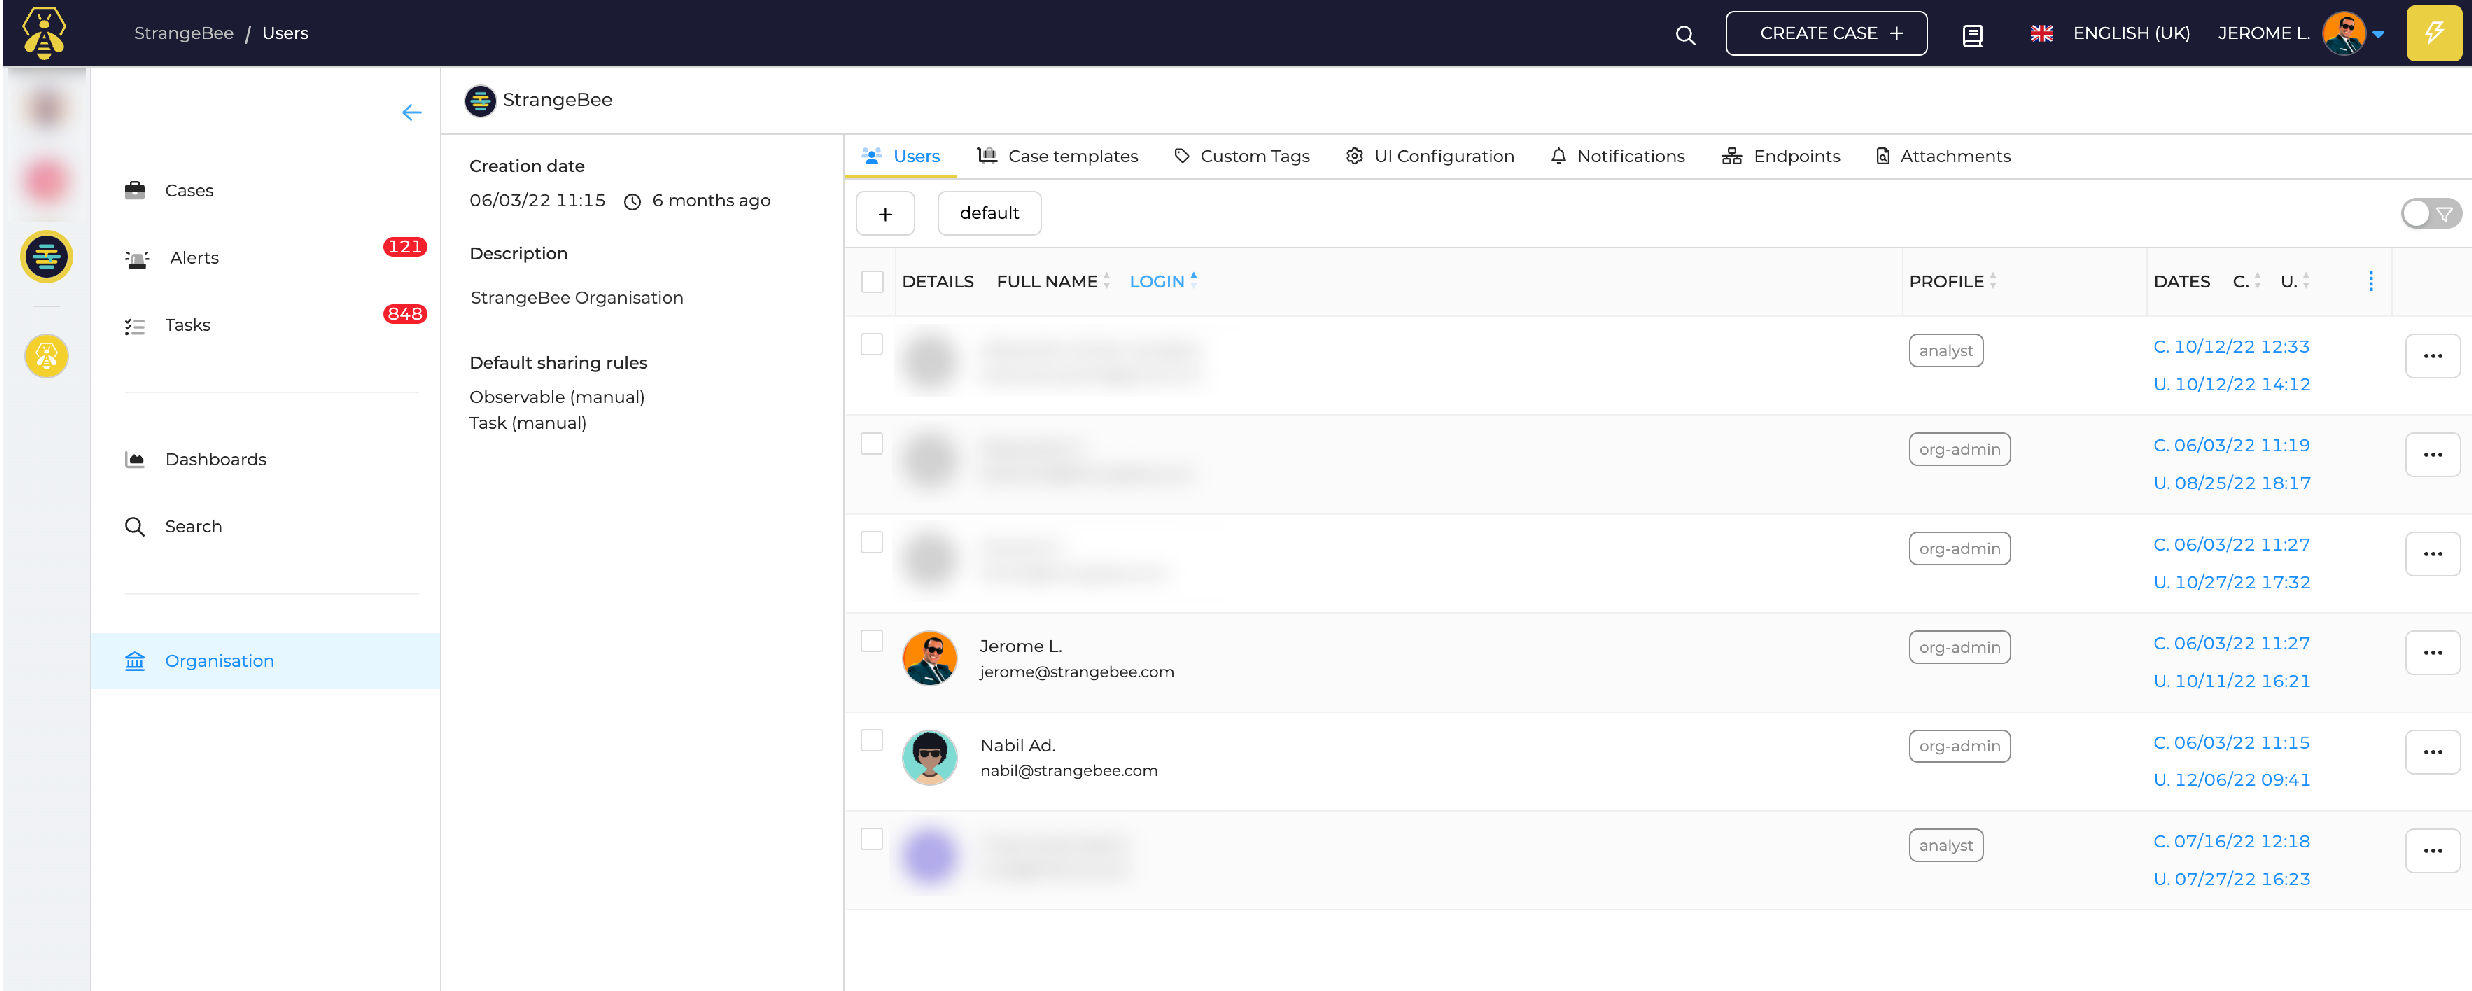
\includegraphics[width=467.99pt,height=187.62pt]{latexImage_cc678f2c180a76dd35f41122226ad91d.png}}
\put(224.195,-267.95){\fontsize{9.9626}{1}\usefont{T1}{cmr}{m}{n}\selectfont\color{color_29791}Figure}
\put(57,-913.465){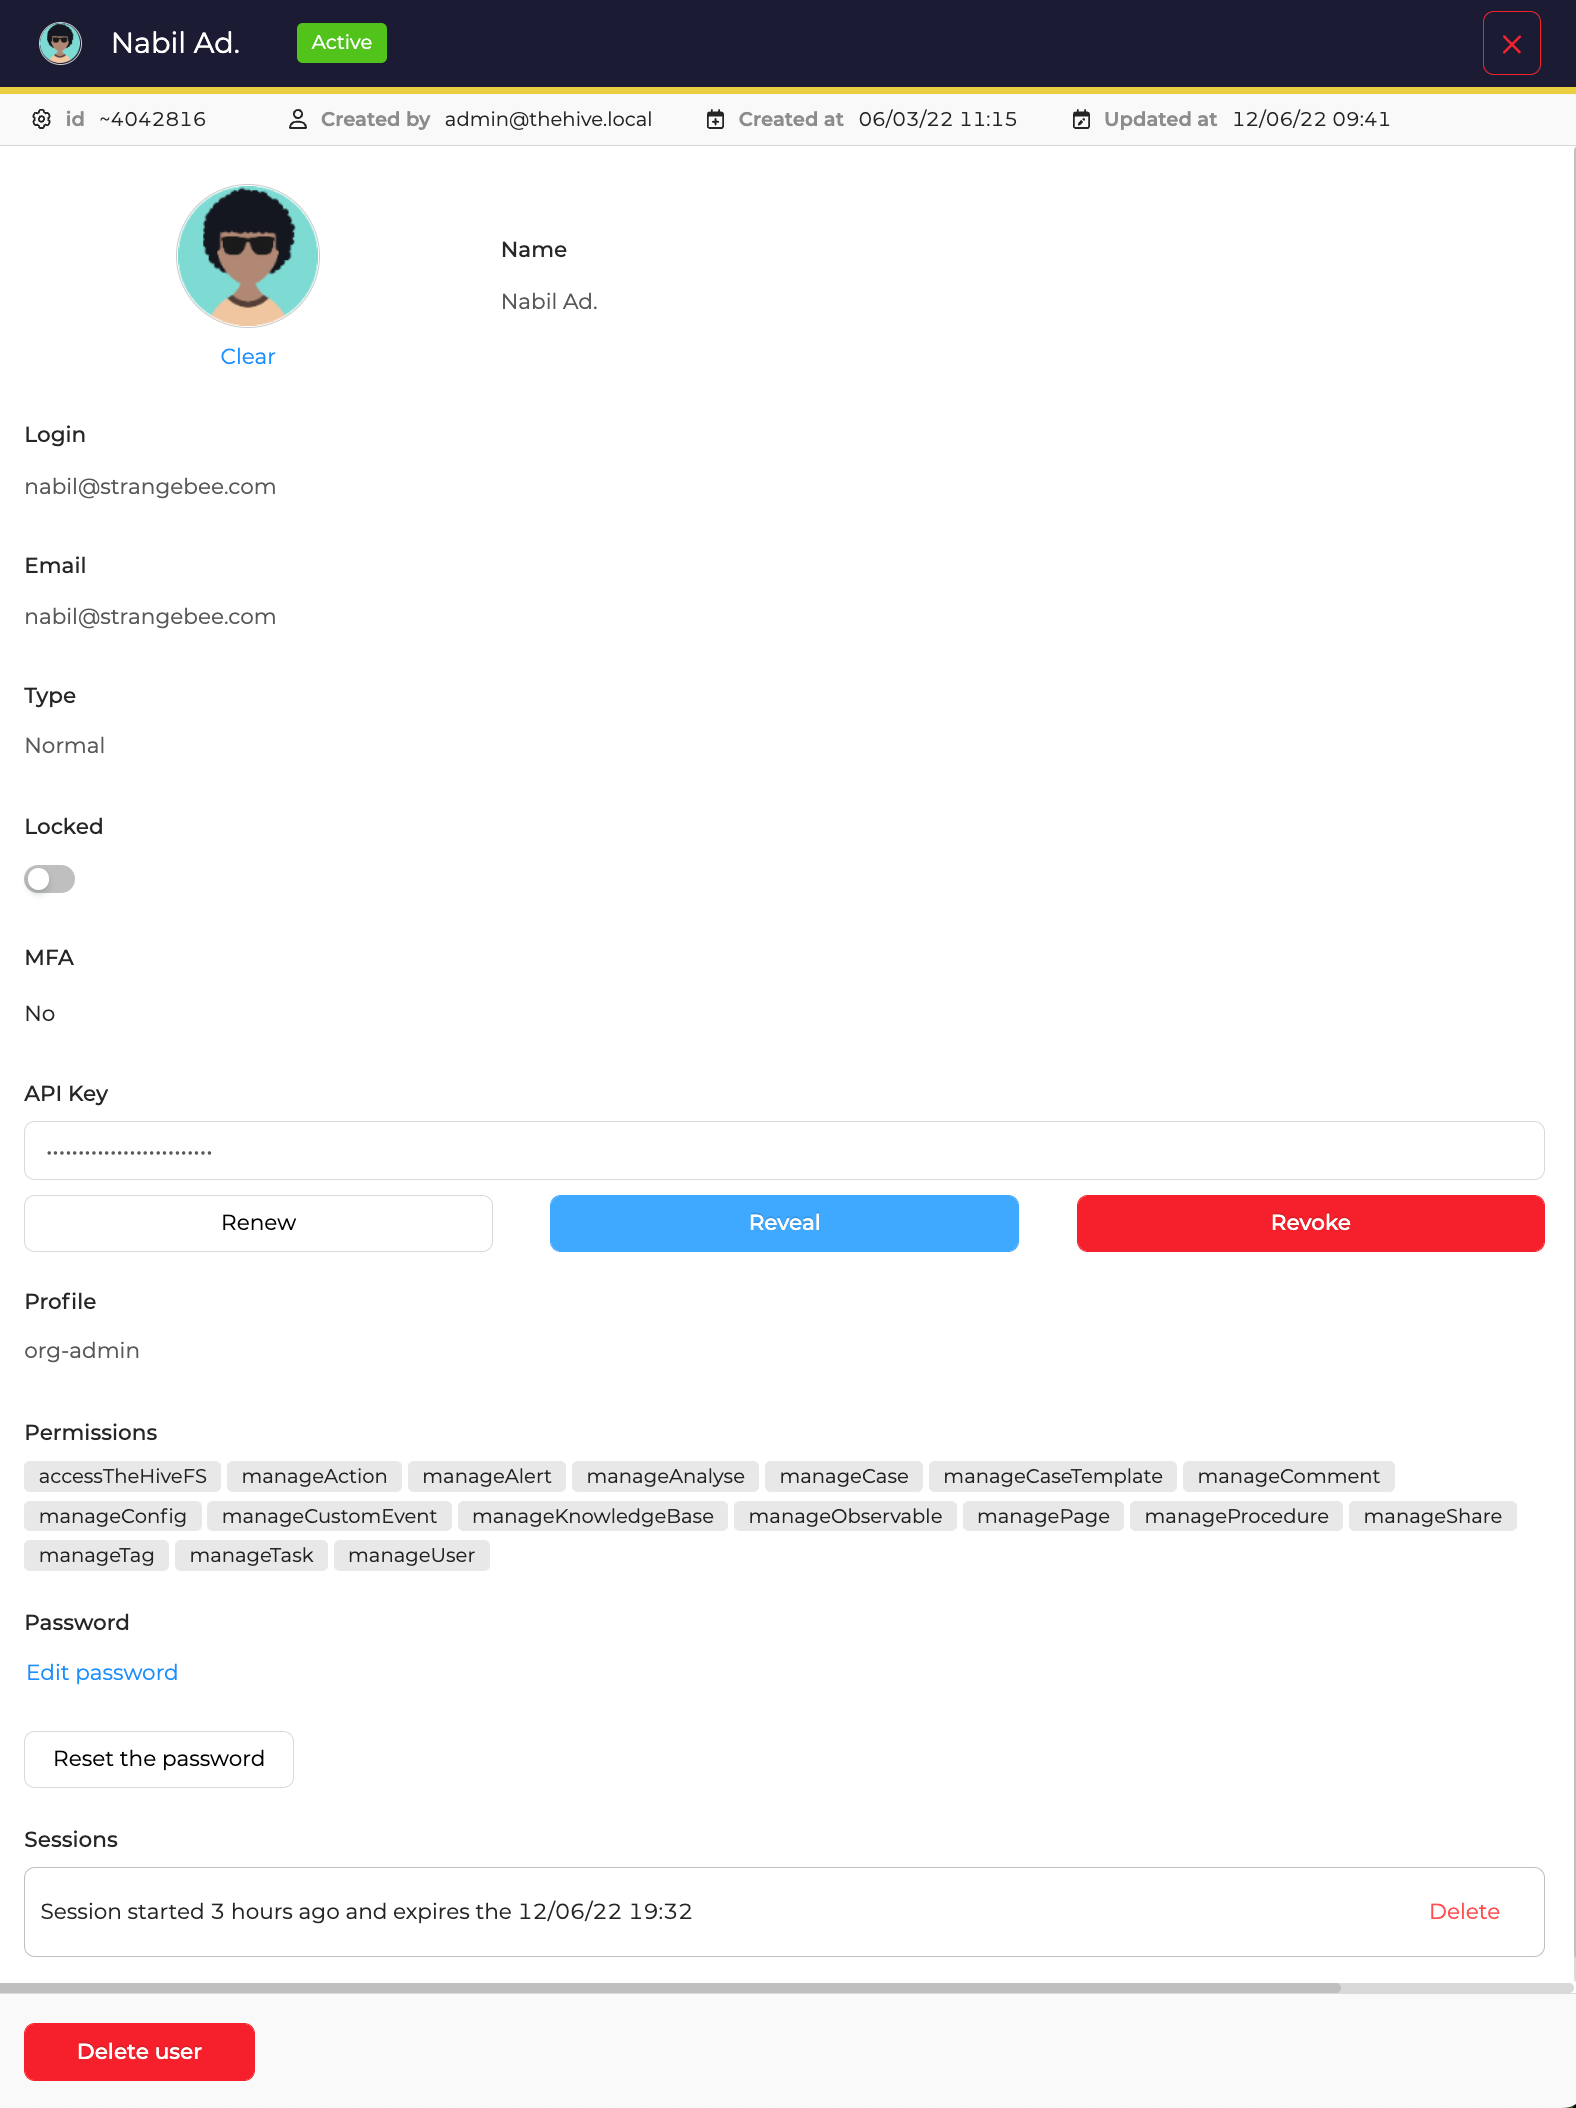
\includegraphics[width=468.0089pt,height=625.9917pt]{latexImage_37ba3b00e4ef419c2e5a2fcb0e365931.png}}
\put(232.331,-931.796){\fontsize{9.9626}{1}\usefont{T1}{cmr}{m}{n}\selectfont\color{color_29791}Figure 3: User information}
\end{picture}

\newpage
\begin{picture}(-5,0)(2.5,0)
\put(57,-71.96301){\fontsize{9.9626}{1}\usefont{T1}{cmr}{b}{n}\selectfont\color{color_29791}Configuration parameters}
\put(71.945,-89.89502){\fontsize{9.9626}{1}\usefont{T1}{cmr}{m}{n}\selectfont\color{color_29791}• Avatar : Up date the avatar associated with the user by drag and drop a new file (PNG or JPG files).}
\put(71.945,-101.851){\fontsize{9.9626}{1}\usefont{T1}{cmr}{m}{n}\selectfont\color{color_29791}• Login : User login}
\put(71.94501,-113.806){\fontsize{9.9626}{1}\usefont{T1}{cmr}{m}{n}\selectfont\color{color_29791}• Email : email address for the account. This is used to send notifications or reset password links to}
\put(81.90701,-125.761){\fontsize{9.9626}{1}\usefont{T1}{cmr}{m}{n}\selectfont\color{color_29791}users. Login is used if no email is filled there}
\put(71.94501,-137.7161){\fontsize{9.9626}{1}\usefont{T1}{cmr}{m}{n}\selectfont\color{color_29791}• Type : Typ e of the account. Normal or Service. A Service account cannot open interactive session}
\put(71.945,-149.6711){\fontsize{9.9626}{1}\usefont{T1}{cmr}{m}{n}\selectfont\color{color_29791}• Locked : Block a user from logging in the application}
\put(71.94499,-161.6261){\fontsize{9.9626}{1}\usefont{T1}{cmr}{m}{n}\selectfont\color{color_29791}• MFA : Tells if a user has configured MFA or not (Multi Factor Authentication). If yes, Yes is displayed}
\put(71.94499,-173.5821){\fontsize{9.9626}{1}\usefont{T1}{cmr}{m}{n}\selectfont\color{color_29791}• API Key : Define, Renew, Reveal or Revoke API key of the account}
\put(71.94499,-185.5371){\fontsize{9.9626}{1}\usefont{T1}{cmr}{m}{n}\selectfont\color{color_29791}• Profile : Information about the profile given to the user}
\put(71.94499,-197.4921){\fontsize{9.9626}{1}\usefont{T1}{cmr}{m}{n}\selectfont\color{color_29791}• Permissions : List of permissions included in the profile}
\put(71.94498,-209.4471){\fontsize{9.9626}{1}\usefont{T1}{cmr}{m}{n}\selectfont\color{color_29791}• Password : Create or up date the password of the user}
\put(71.94498,-221.4022){\fontsize{9.9626}{1}\usefont{T1}{cmr}{m}{n}\selectfont\color{color_29791}• Reset Password : If the application is configured with a SMTP server, send an email with a magic}
\put(81.90697,-233.3572){\fontsize{9.9626}{1}\usefont{T1}{cmr}{m}{n}\selectfont\color{color_29791}link to the user. link is active for a short time period.}
\put(71.94498,-245.3132){\fontsize{9.9626}{1}\usefont{T1}{cmr}{m}{n}\selectfont\color{color_29791}• Sessions : List of opened interactive sessions. Click delete to close a session}
\put(56.99997,-271.2092){\fontsize{9.9626}{1}\usefont{T1}{cmr}{b}{n}\selectfont\color{color_29791}Add Users}
\put(56.99997,-289.1412){\fontsize{9.9626}{1}\usefont{T1}{cmr}{m}{n}\selectfont\color{color_29791}org-admin}
\put(57,-490.999){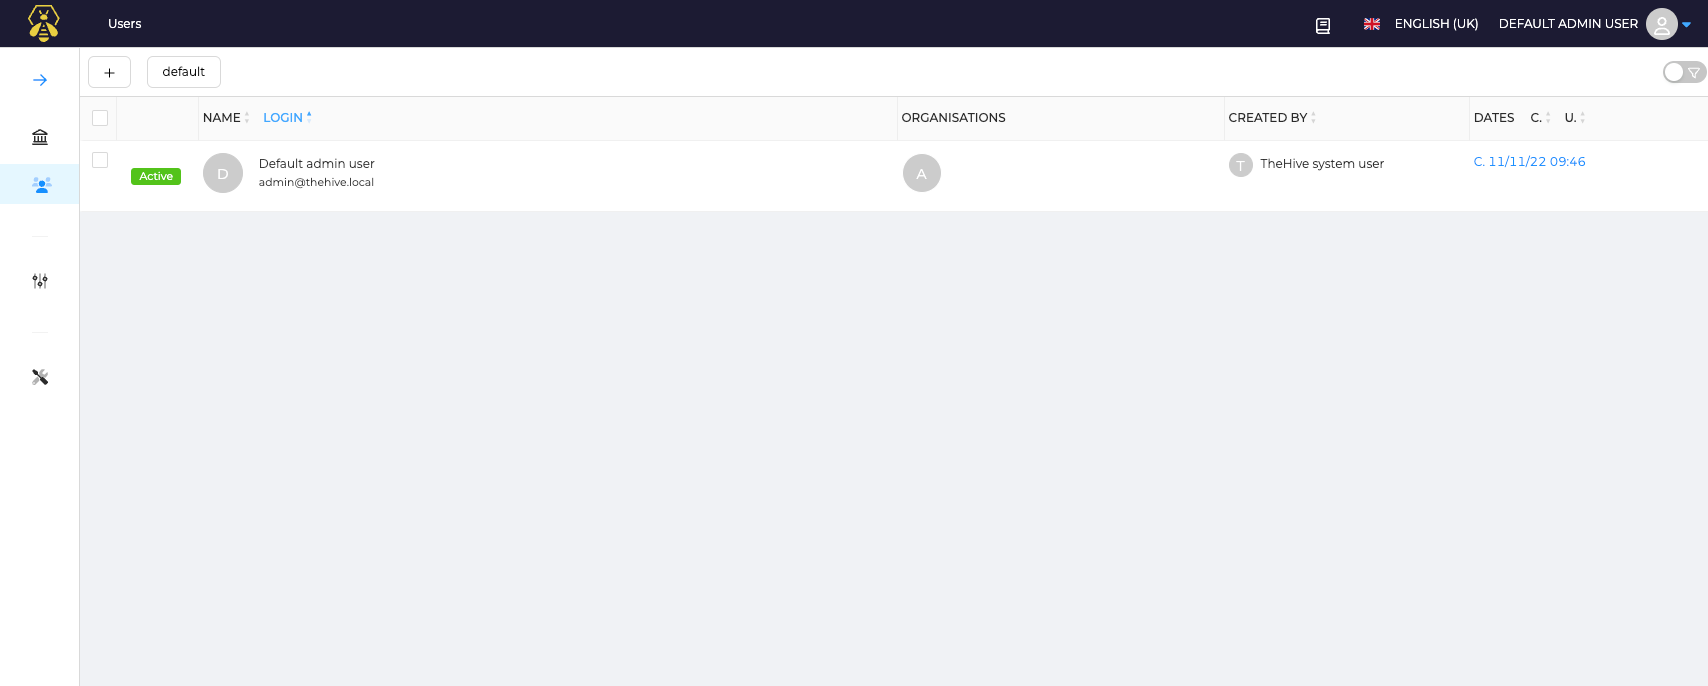
\includegraphics[width=467.9919pt,height=187.964pt]{latexImage_ab1bdaab1861669eaab19c11bfdc0496.png}}
\put(57,-524.927){\fontsize{9.9626}{1}\usefont{T1}{cmr}{m}{n}\selectfont\color{color_29791}Click the + button to add an account in the current organisation, and follow create an account and up date}
\put(57,-536.882){\fontsize{9.9626}{1}\usefont{T1}{cmr}{m}{n}\selectfont\color{color_29791}an account guides.}
\end{picture}
\begin{tikzpicture}[overlay]
\path(0pt,0pt);
\draw[color_29791,line width=0.996pt]
(57pt, -727.435pt) -- (525pt, -727.435pt)
;
\end{tikzpicture}
\begin{picture}(-5,0)(2.5,0)
\put(519.521,-739.888){\fontsize{9.9626}{1}\usefont{T1}{cmr}{b}{n}\selectfont\color{color_29791}8}
\end{picture}
\newpage

\begin{picture}(-5,0)(2.5,0)
\put(57,-332.856){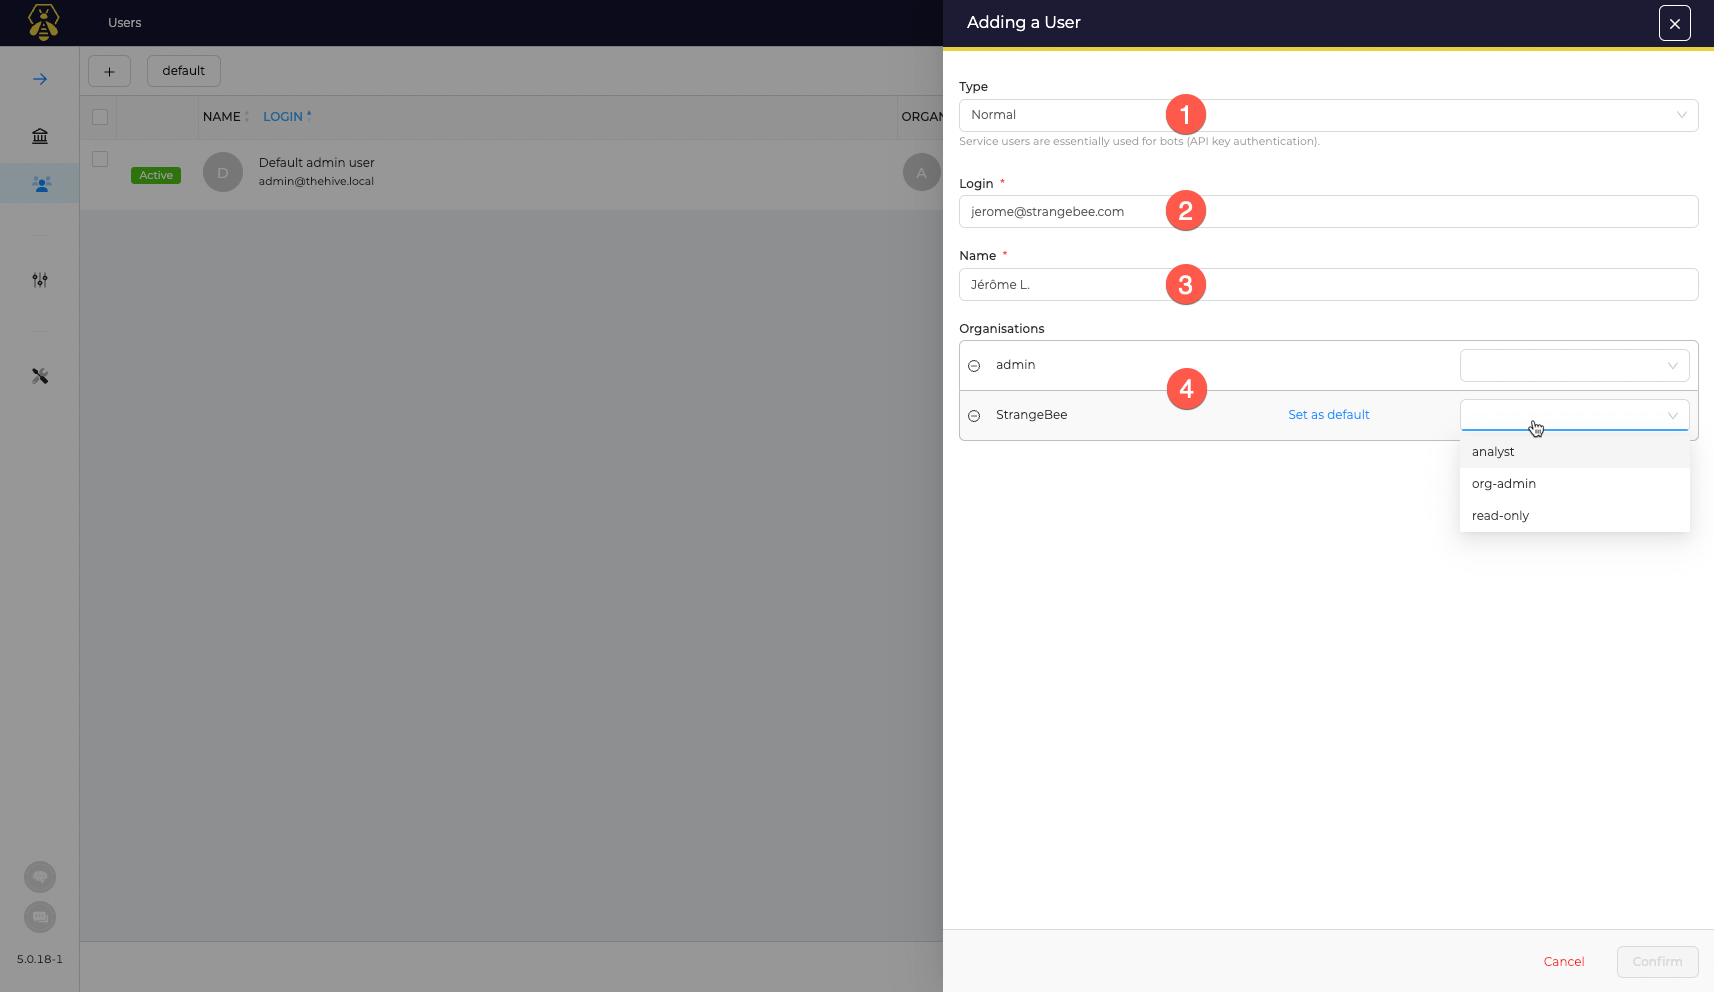
\includegraphics[width=467.9905pt,height=270.8557pt]{latexImage_22bea9efecc92b029dfb2d8dbdc8a614.png}}
\put(57,-374.699){\fontsize{9.9626}{1}\usefont{T1}{cmr}{m}{n}\selectfont\color{color_29791}In the list of accounts, click Preview to open accounts details view}
\put(57,-685.364){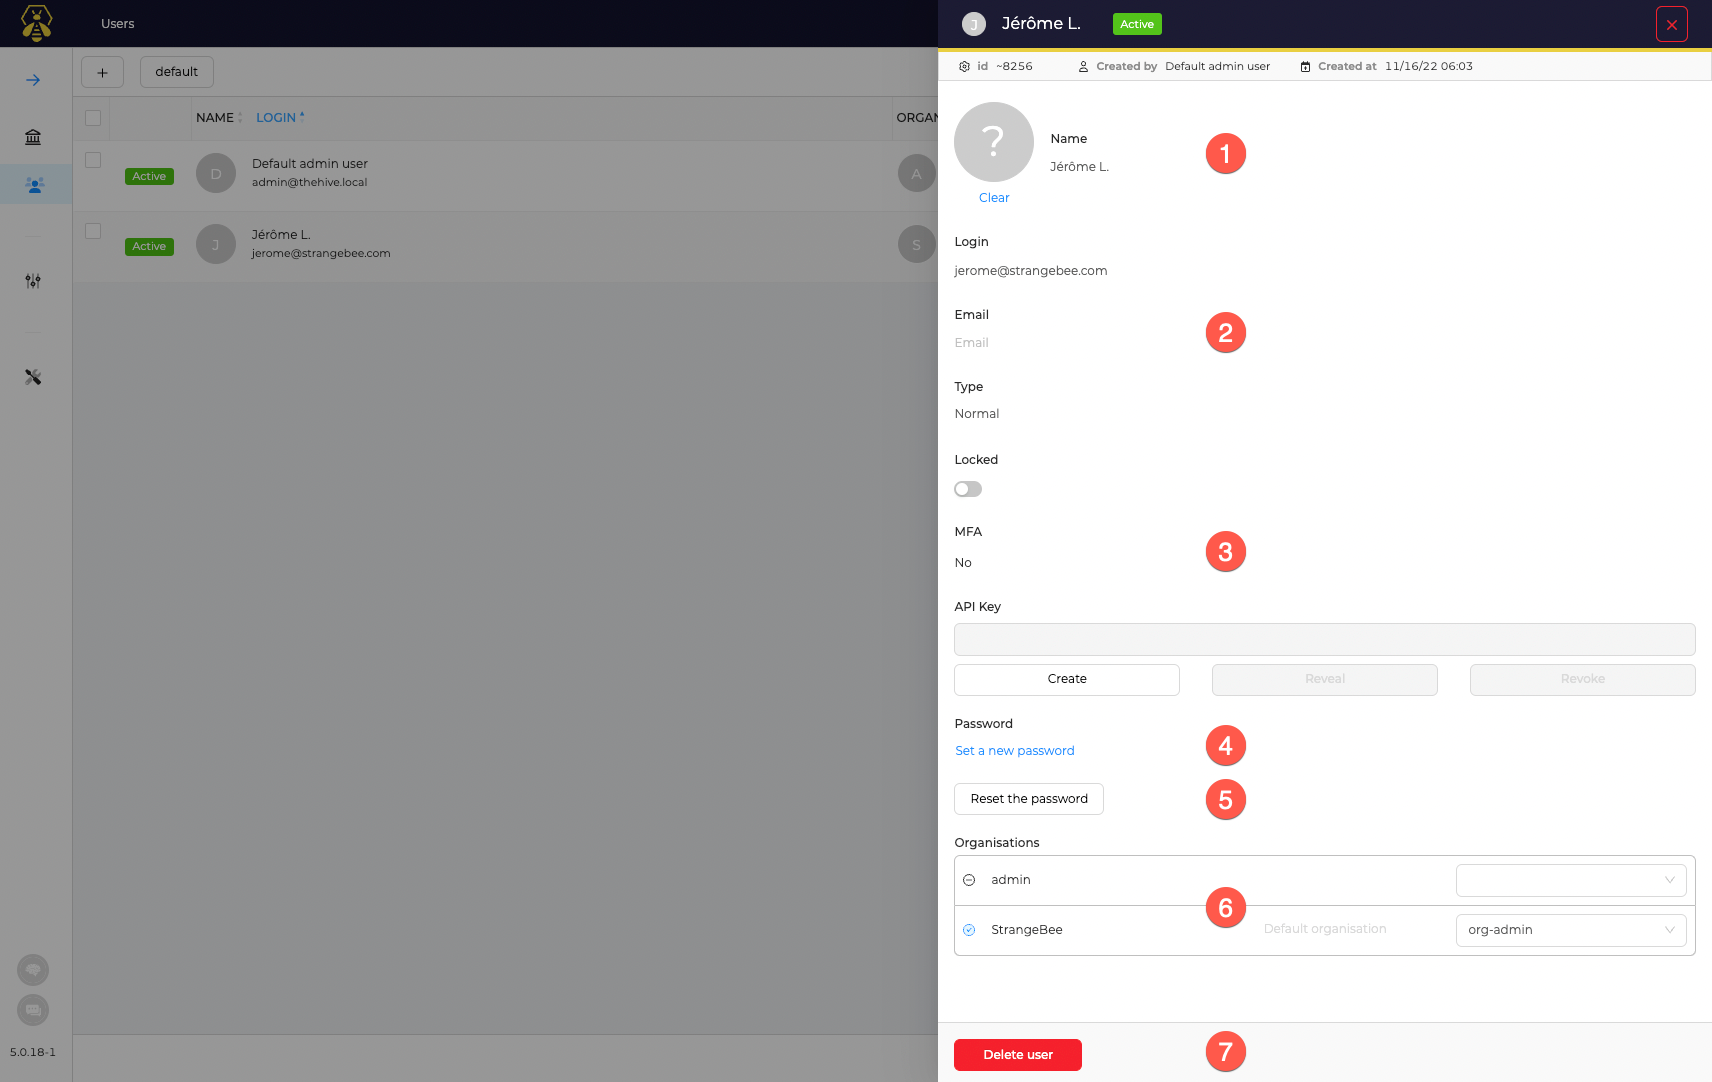
\includegraphics[width=467.9923pt,height=295.7755pt]{latexImage_b63bb41705e4dc5aa411e4cbfaaf0ffd.png}}
\end{picture}
\begin{tikzpicture}[overlay]
\path(0pt,0pt);
\draw[color_29791,line width=0.996pt]
(57pt, -727.435pt) -- (525pt, -727.435pt)
;
\end{tikzpicture}
\begin{picture}(-5,0)(2.5,0)

\put(519.521,-739.888){\fontsize{9.9626}{1}\usefont{T1}{cmr}{b}{n}\selectfont\color{color_29791}9}
\end{picture}
\newpage

\begin{picture}(-5,0)(2.5,0)
\put(57,-71.96301){\fontsize{9.9626}{1}\usefont{T1}{cmr}{b}{n}\selectfont\color{color_29791}5.1.2 Templates}
\put(71.945,-90.35199){\fontsize{9.9626}{1}\usefont{T1}{cmr}{m}{n}\selectfont\color{color_29791}• Case}
\put(81.907,-116.248){\fontsize{9.9626}{1}\usefont{T1}{cmr}{b}{n}\selectfont\color{color_29791}List of Case Templates}
\put(81.907,-134.181){\fontsize{9.9626}{1}\usefont{T1}{cmr}{m}{n}\selectfont\color{color_29791}Access}
\put(57,-375.869){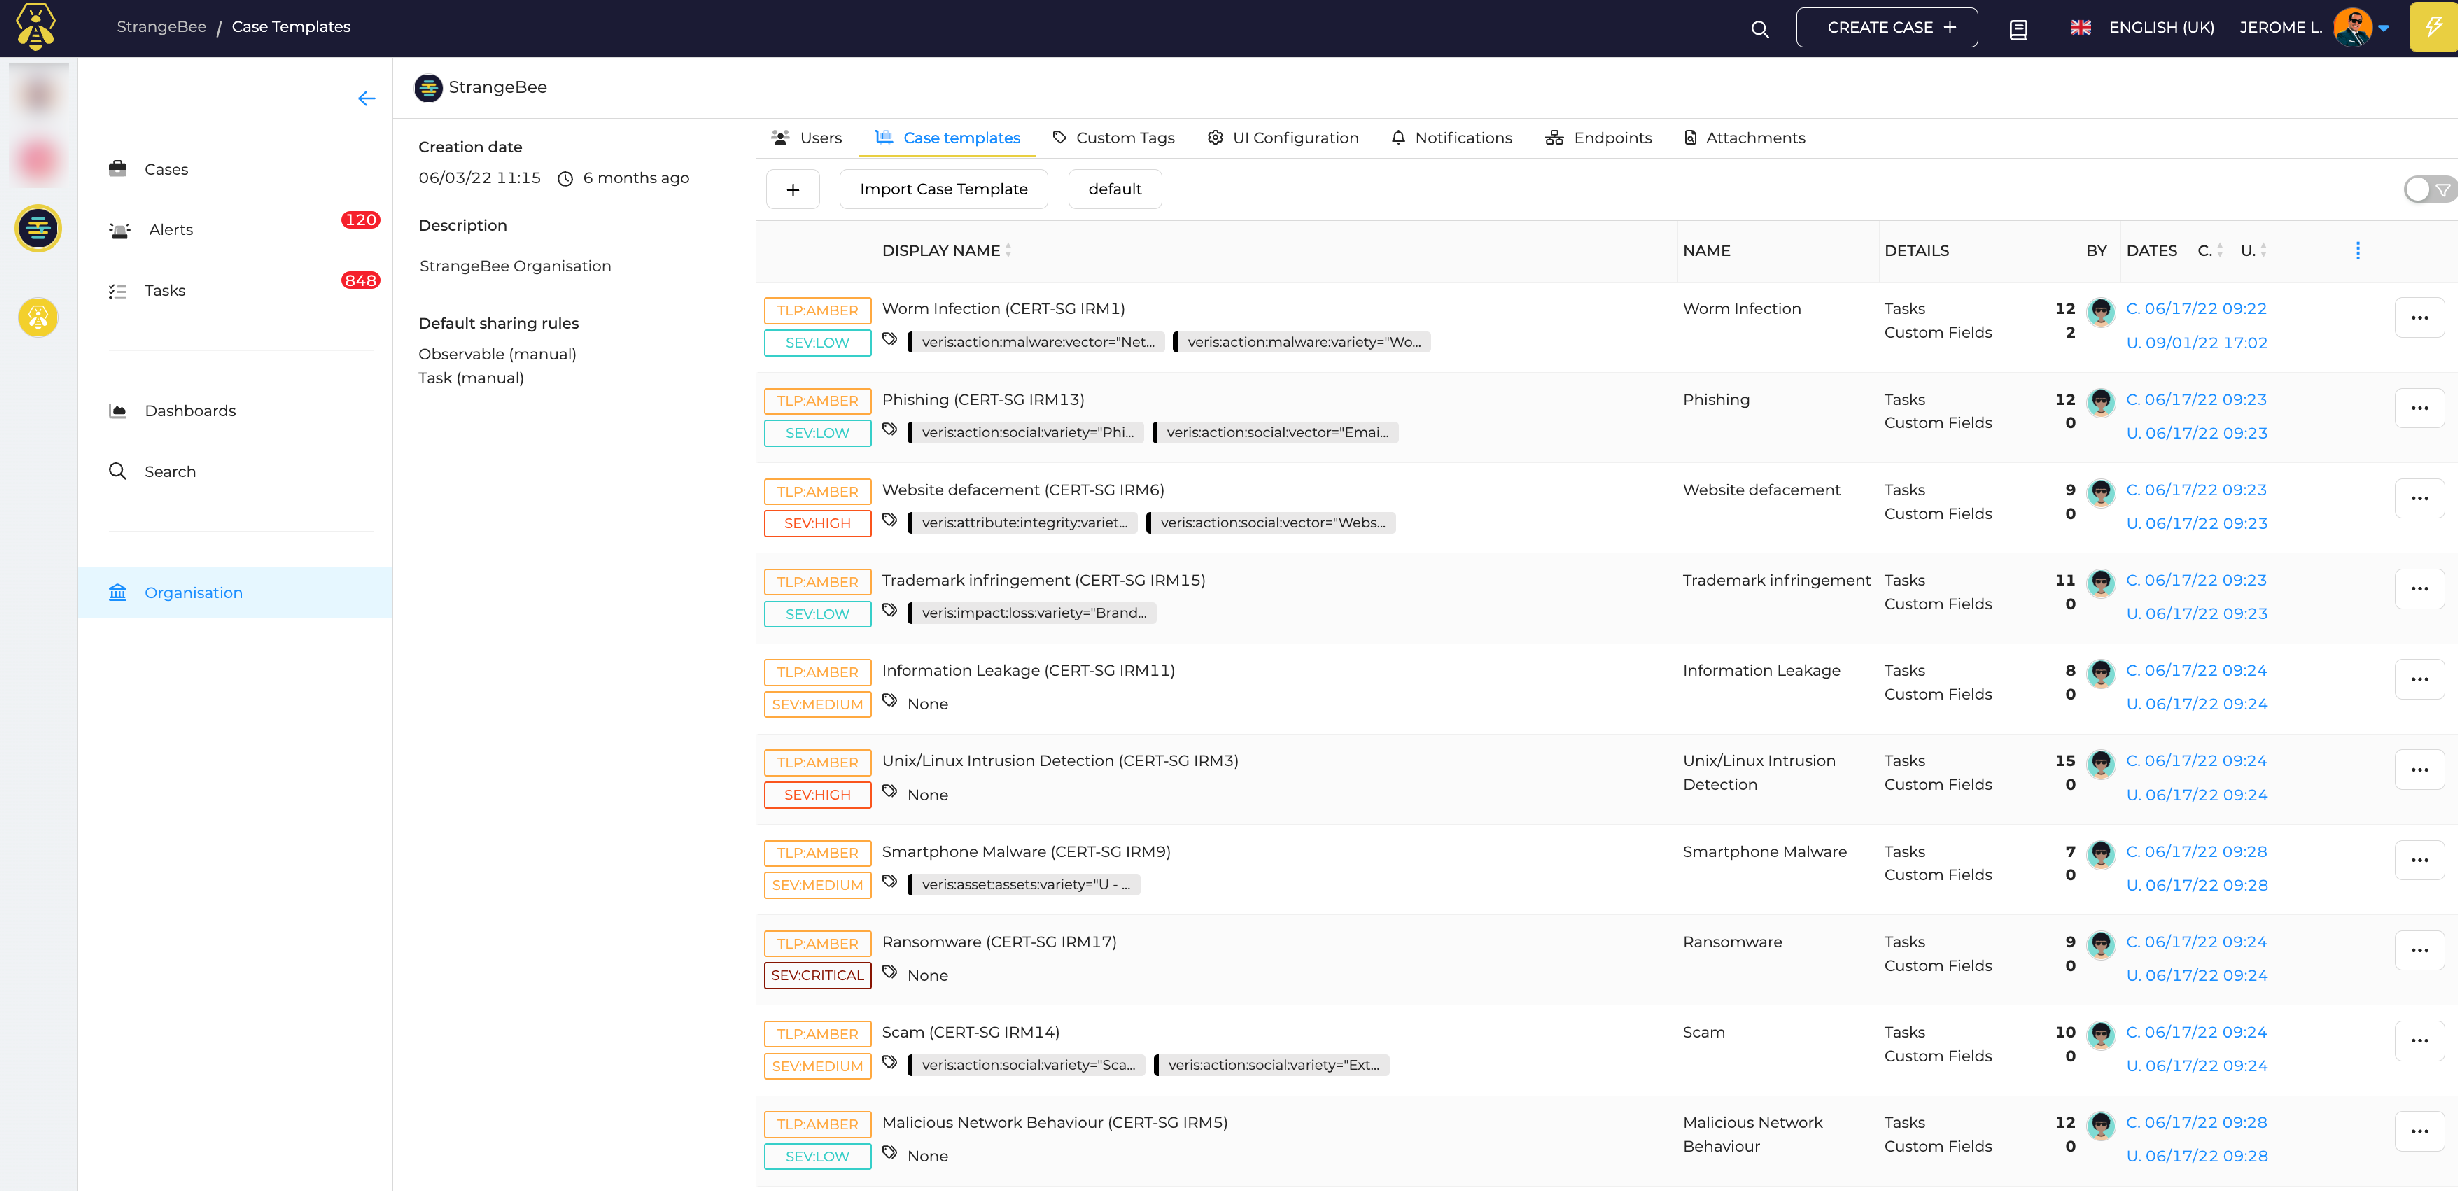
\includegraphics[width=467.9916pt,height=226.8pt]{latexImage_c14153f4daf94fb96d1bd60b49ac2ccb.png}}
\put(221.856,-394.2){\fontsize{9.9626}{1}\usefont{T1}{cmr}{m}{n}\selectfont\color{color_29791}Figure 4: List of case templates}
\put(81.907,-427.674){\fontsize{9.9626}{1}\usefont{T1}{cmr}{b}{n}\selectfont\color{color_29791}New Case template}
\put(81.907,-445.607){\fontsize{9.9626}{1}\usefont{T1}{cmr}{m}{n}\selectfont\color{color_29791}Click the + button to create a new Case template.}
\end{picture}
\begin{tikzpicture}[overlay]
\path(0pt,0pt);
\draw[color_29791,line width=0.996pt]
(57pt, -727.435pt) -- (525pt, -727.435pt)
;
\end{tikzpicture}
\begin{picture}(-5,0)(2.5,0)
\put(514.041,-739.888){\fontsize{9.9626}{1}\usefont{T1}{cmr}{b}{n}\selectfont\color{color_29791}10}
\end{picture}
\newpage

\begin{picture}(-5,0)(2.5,0)
\put(57,-538.762){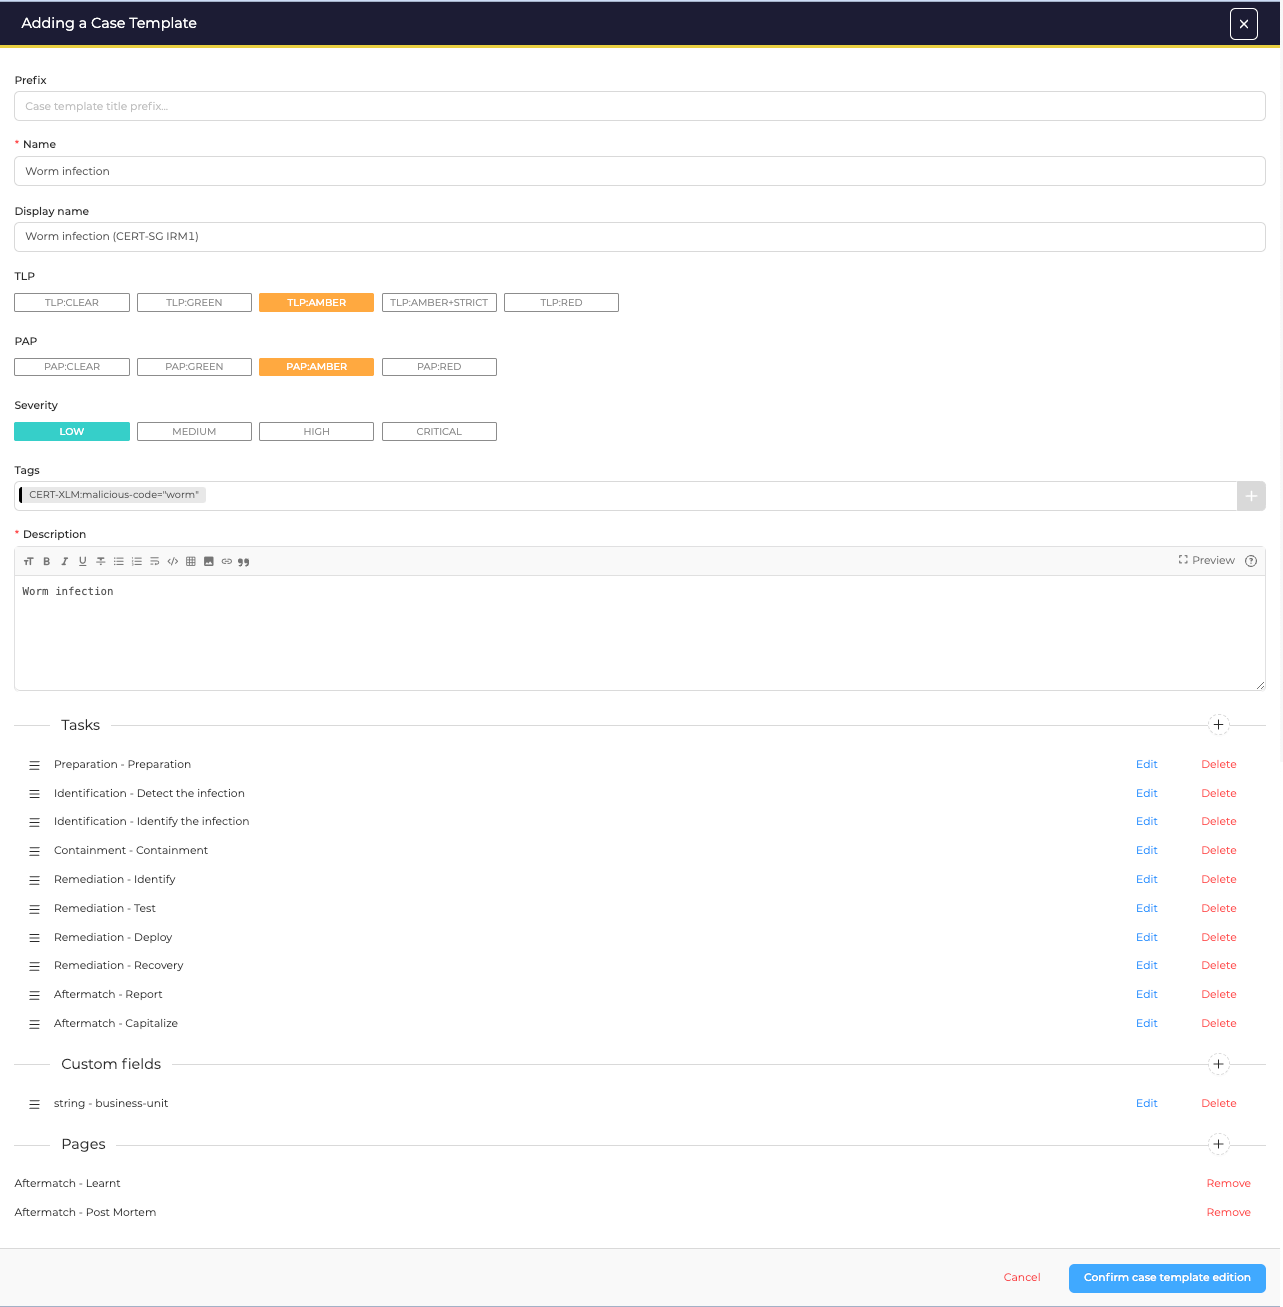
\includegraphics[width=468.0128pt,height=476.7675pt]{latexImage_fbfc54efb85496b1f2f4e885f34a9c02.png}}
\put(228.346,-557.093){\fontsize{9.9626}{1}\usefont{T1}{cmr}{m}{n}\selectfont\color{color_29791}Figure 5: New case template}
\put(81.907,-590.568){\fontsize{9.9626}{1}\usefont{T1}{cmr}{b}{n}\selectfont\color{color_29791}Configuration parameters}
\put(93.115,-608.5){\fontsize{9.9626}{1}\usefont{T1}{cmr}{b}{n}\selectfont\color{color_29791}–}
\put(98.84349,-608.5){\fontsize{9.9626}{1}\usefont{T1}{cmr}{b}{n}\selectfont\color{color_29791}}
\put(103.8248,-608.5){\fontsize{9.9626}{1}\usefont{T1}{cmr}{b}{n}\selectfont\color{color_29791}Prefix : String that will b e prepended to the title of a Case when created with this template}
\put(93.11501,-620.456){\fontsize{9.9626}{1}\usefont{T1}{cmr}{b}{n}\selectfont\color{color_29791}–}
\put(98.8435,-620.456){\fontsize{9.9626}{1}\usefont{T1}{cmr}{b}{n}\selectfont\color{color_29791}}
\put(103.8248,-620.456){\fontsize{9.9626}{1}\usefont{T1}{cmr}{b}{n}\selectfont\color{color_29791}Name : Name of the Case template. Used to identify the Case template with the API}
\put(93.11501,-632.411){\fontsize{9.9626}{1}\usefont{T1}{cmr}{b}{n}\selectfont\color{color_29791}–}
\put(98.8435,-632.411){\fontsize{9.9626}{1}\usefont{T1}{cmr}{b}{n}\selectfont\color{color_29791}}
\put(103.8248,-632.411){\fontsize{9.9626}{1}\usefont{T1}{cmr}{b}{n}\selectfont\color{color_29791}Display Name : Name of the Case template displayed in the UI}
\put(93.11501,-644.366){\fontsize{9.9626}{1}\usefont{T1}{cmr}{b}{n}\selectfont\color{color_29791}–}
\put(98.8435,-644.366){\fontsize{9.9626}{1}\usefont{T1}{cmr}{b}{n}\selectfont\color{color_29791}}
\put(103.8248,-644.366){\fontsize{9.9626}{1}\usefont{T1}{cmr}{b}{n}\selectfont\color{color_29791}TLP : Default TLP of the Case when created with this template}
\put(93.11501,-656.321){\fontsize{9.9626}{1}\usefont{T1}{cmr}{b}{n}\selectfont\color{color_29791}–}
\put(98.84351,-656.321){\fontsize{9.9626}{1}\usefont{T1}{cmr}{b}{n}\selectfont\color{color_29791}}
\put(103.8248,-656.321){\fontsize{9.9626}{1}\usefont{T1}{cmr}{b}{n}\selectfont\color{color_29791}PAP : Default PAP o f the Case when created with this template}
\put(93.11502,-668.276){\fontsize{9.9626}{1}\usefont{T1}{cmr}{b}{n}\selectfont\color{color_29791}–}
\put(98.84351,-668.276){\fontsize{9.9626}{1}\usefont{T1}{cmr}{b}{n}\selectfont\color{color_29791}}
\put(103.8248,-668.276){\fontsize{9.9626}{1}\usefont{T1}{cmr}{b}{n}\selectfont\color{color_29791}Severity : Default Severity of the Case when created with this template}
\put(93.11502,-680.231){\fontsize{9.9626}{1}\usefont{T1}{cmr}{b}{n}\selectfont\color{color_29791}–}
\put(98.84351,-680.231){\fontsize{9.9626}{1}\usefont{T1}{cmr}{b}{n}\selectfont\color{color_29791}}
\put(103.8248,-680.231){\fontsize{9.9626}{1}\usefont{T1}{cmr}{b}{n}\selectfont\color{color_29791}Tags : List of tags that will be added to the Cases created with this template}
\put(93.11503,-692.187){\fontsize{9.9626}{1}\usefont{T1}{cmr}{b}{n}\selectfont\color{color_29791}–}
\put(98.84352,-692.187){\fontsize{9.9626}{1}\usefont{T1}{cmr}{b}{n}\selectfont\color{color_29791}}
\put(103.8248,-692.187){\fontsize{9.9626}{1}\usefont{T1}{cmr}{b}{n}\selectfont\color{color_29791}Description : Default description of Cases created with this template if not modified .}
\put(93.11503,-704.142){\fontsize{9.9626}{1}\usefont{T1}{cmr}{b}{n}\selectfont\color{color_29791}–}
\put(98.84352,-704.142){\fontsize{9.9626}{1}\usefont{T1}{cmr}{b}{n}\selectfont\color{color_29791}}
\put(103.8248,-704.142){\fontsize{9.9626}{1}\usefont{T1}{cmr}{b}{n}\selectfont\color{color_29791}Tasks : Add tasks to the templates. They will be automatically added to the Case when created}
\end{picture}
\begin{tikzpicture}[overlay]
\path(0pt,0pt);
\draw[color_29791,line width=0.996pt]
(57pt, -727.435pt) -- (525pt, -727.435pt)
;
\end{tikzpicture}
\begin{picture}(-5,0)(2.5,0)
\put(514.041,-739.888){\fontsize{9.9626}{1}\usefont{T1}{cmr}{b}{n}\selectfont\color{color_29791}11}
\end{picture}
\newpage
\begin{picture}(-5,0)(2.5,0)
\put(103.824,-71.96301){\fontsize{9.9626}{1}\usefont{T1}{cmr}{m}{n}\selectfont\color{color_29791}with this template}
\put(93.115,-83.91803){\fontsize{9.9626}{1}\usefont{T1}{cmr}{b}{n}\selectfont\color{color_29791}–}
\put(98.84349,-83.91803){\fontsize{9.9626}{1}\usefont{T1}{cmr}{b}{n}\selectfont\color{color_29791}}
\put(103.8248,-83.91803){\fontsize{9.9626}{1}\usefont{T1}{cmr}{b}{n}\selectfont\color{color_29791}Custom Fields : Add Custom fields to the template. Default value can b e set for Custom fields}
\put(103.824,-95.87305){\fontsize{9.9626}{1}\usefont{T1}{cmr}{m}{n}\selectfont\color{color_29791}as well.}
\put(93.11501,-107.8281){\fontsize{9.9626}{1}\usefont{T1}{cmr}{b}{n}\selectfont\color{color_29791}–}
\put(98.8435,-107.8281){\fontsize{9.9626}{1}\usefont{T1}{cmr}{b}{n}\selectfont\color{color_29791}}
\put(103.8248,-107.8281){\fontsize{9.9626}{1}\usefont{T1}{cmr}{b}{n}\selectfont\color{color_29791}Pages : Add pages template to the template. They will be automatically added to the Case}
\put(103.824,-119.7831){\fontsize{9.9626}{1}\usefont{T1}{cmr}{m}{n}\selectfont\color{color_29791}when created with this template}
\put(71.94501,-137.7161){\fontsize{9.9626}{1}\usefont{T1}{cmr}{m}{n}\selectfont\color{color_29791}• Pages}
\put(81.90701,-163.6121){\fontsize{9.9626}{1}\usefont{T1}{cmr}{b}{n}\selectfont\color{color_29791}List of Page Templates}
\put(81.90701,-181.545){\fontsize{9.9626}{1}\usefont{T1}{cmr}{m}{n}\selectfont\color{color_29791}Access}
\put(57,-349.039){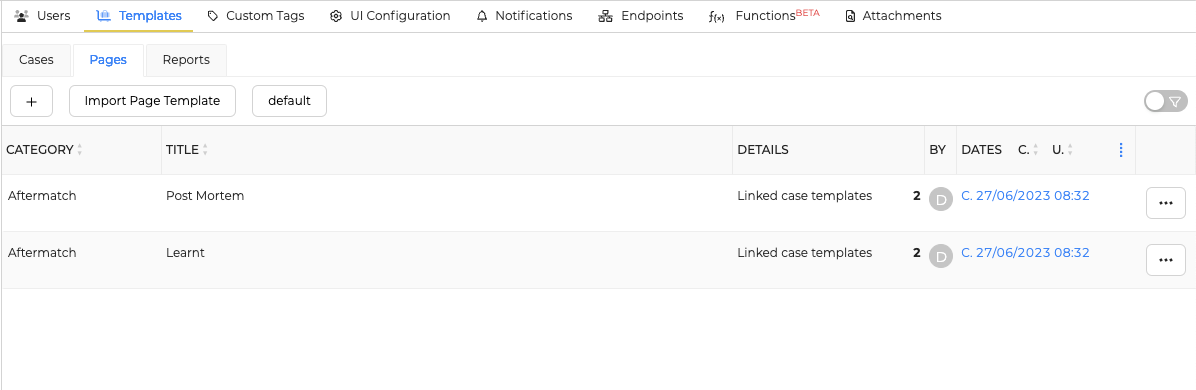
\includegraphics[width=467.9948pt,height=152.607pt]{latexImage_a5723fc8ab02f6fcc055d7f02fc3b780.png}}
\put(218.812,-367.37){\fontsize{9.9626}{1}\usefont{T1}{cmr}{m}{n}\selectfont\color{color_29791}Figure 6: List of pages templates}
\put(81.907,-400.844){\fontsize{9.9626}{1}\usefont{T1}{cmr}{b}{n}\selectfont\color{color_29791}New Case template}
\put(81.907,-418.777){\fontsize{9.9626}{1}\usefont{T1}{cmr}{m}{n}\selectfont\color{color_29791}Click the + button to create a new Page template.}
\end{picture}
\begin{tikzpicture}[overlay]
\path(0pt,0pt);
\draw[color_29791,line width=0.996pt]
(57pt, -727.435pt) -- (525pt, -727.435pt)
;
\end{tikzpicture}
\begin{picture}(-5,0)(2.5,0)

\put(514.041,-739.888){\fontsize{9.9626}{1}\usefont{T1}{cmr}{b}{n}\selectfont\color{color_29791}12}
\end{picture}
\newpage

\begin{picture}(-5,0)(2.5,0)
\put(57,-384.567){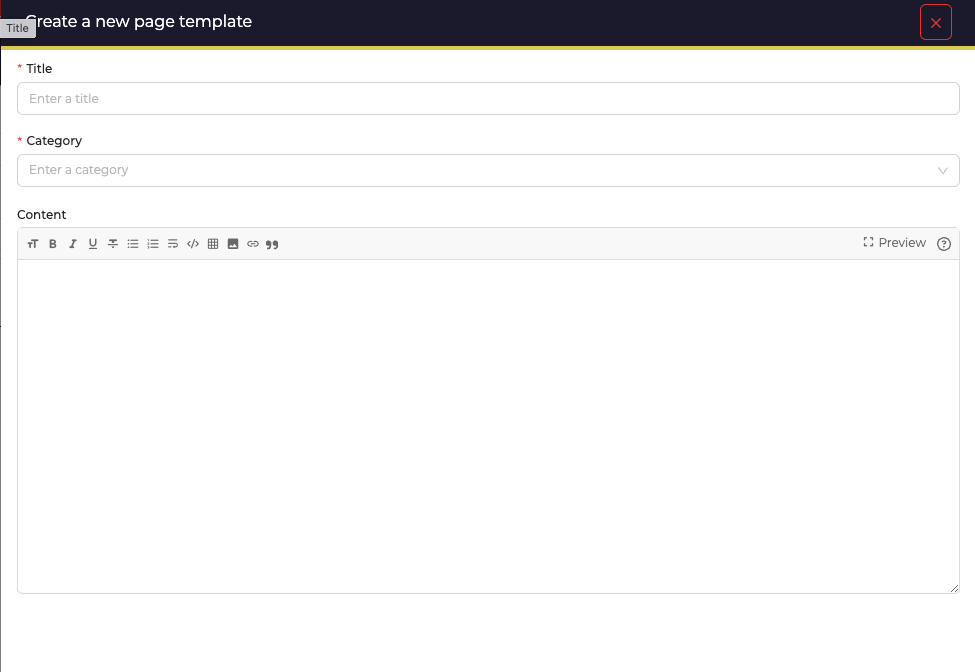
\includegraphics[width=468.0098pt,height=322.5667pt]{latexImage_8f51d0c0a48b341eed002c023c4e42b5.png}}
\put(226.782,-402.898){\fontsize{9.9626}{1}\usefont{T1}{cmr}{m}{n}\selectfont\color{color_29791}Figure 7: New P age template}
\put(81.907,-436.372){\fontsize{9.9626}{1}\usefont{T1}{cmr}{b}{n}\selectfont\color{color_29791}Configuration parameters}
\put(93.115,-454.305){\fontsize{9.9626}{1}\usefont{T1}{cmr}{b}{n}\selectfont\color{color_29791}–}
\put(98.84349,-454.305){\fontsize{9.9626}{1}\usefont{T1}{cmr}{b}{n}\selectfont\color{color_29791}}
\put(103.8248,-454.305){\fontsize{9.9626}{1}\usefont{T1}{cmr}{b}{n}\selectfont\color{color_29791}Title : Page template title. Used to identify the Page template with the API. Al s o used as a}
\put(103.824,-466.26){\fontsize{9.9626}{1}\usefont{T1}{cmr}{m}{n}\selectfont\color{color_29791}page title when the template is used in a case.}
\put(93.115,-478.215){\fontsize{9.9626}{1}\usefont{T1}{cmr}{b}{n}\selectfont\color{color_29791}–}
\put(98.84349,-478.215){\fontsize{9.9626}{1}\usefont{T1}{cmr}{b}{n}\selectfont\color{color_29791}}
\put(103.8248,-478.215){\fontsize{9.9626}{1}\usefont{T1}{cmr}{b}{n}\selectfont\color{color_29791}Category : Category for grouping pages on a common theme is used as a page tree in the case}
\put(103.824,-490.171){\fontsize{9.9626}{1}\usefont{T1}{cmr}{m}{n}\selectfont\color{color_29791}of.}
\put(93.11499,-502.126){\fontsize{9.9626}{1}\usefont{T1}{cmr}{b}{n}\selectfont\color{color_29791}–}
\put(98.84348,-502.126){\fontsize{9.9626}{1}\usefont{T1}{cmr}{b}{n}\selectfont\color{color_29791}}
\put(103.8248,-502.126){\fontsize{9.9626}{1}\usefont{T1}{cmr}{b}{n}\selectfont\color{color_29791}Content : Default page conten t when the page template is used in a case.}
\end{picture}
\begin{tikzpicture}[overlay]
\path(0pt,0pt);
\draw[color_29791,line width=0.996pt]
(57pt, -727.435pt) -- (525pt, -727.435pt)
;
\end{tikzpicture}
\begin{picture}(-5,0)(2.5,0)

\put(514.041,-739.888){\fontsize{9.9626}{1}\usefont{T1}{cmr}{b}{n}\selectfont\color{color_29791}13}
\end{picture}
\newpage

\begin{picture}(-5,0)(2.5,0)
\put(57,-71.96301){\fontsize{9.9626}{1}\usefont{T1}{cmr}{b}{n}\selectfont\color{color_29791}5.1.3 Tags}
\put(57,-90.35199){\fontsize{9.9626}{1}\usefont{T1}{cmr}{b}{n}\selectfont\color{color_29791}Custom tags}
\put(57,-108.285){\fontsize{9.9626}{1}\usefont{T1}{cmr}{m}{n}\selectfont\color{color_29791}Custom tags collect all tags from Alerts or added to Cases or Observables that are not included in TheHive}
\put(57,-120.24){\fontsize{9.9626}{1}\usefont{T1}{cmr}{m}{n}\selectfont\color{color_29791}T}
\put(57,-317.101){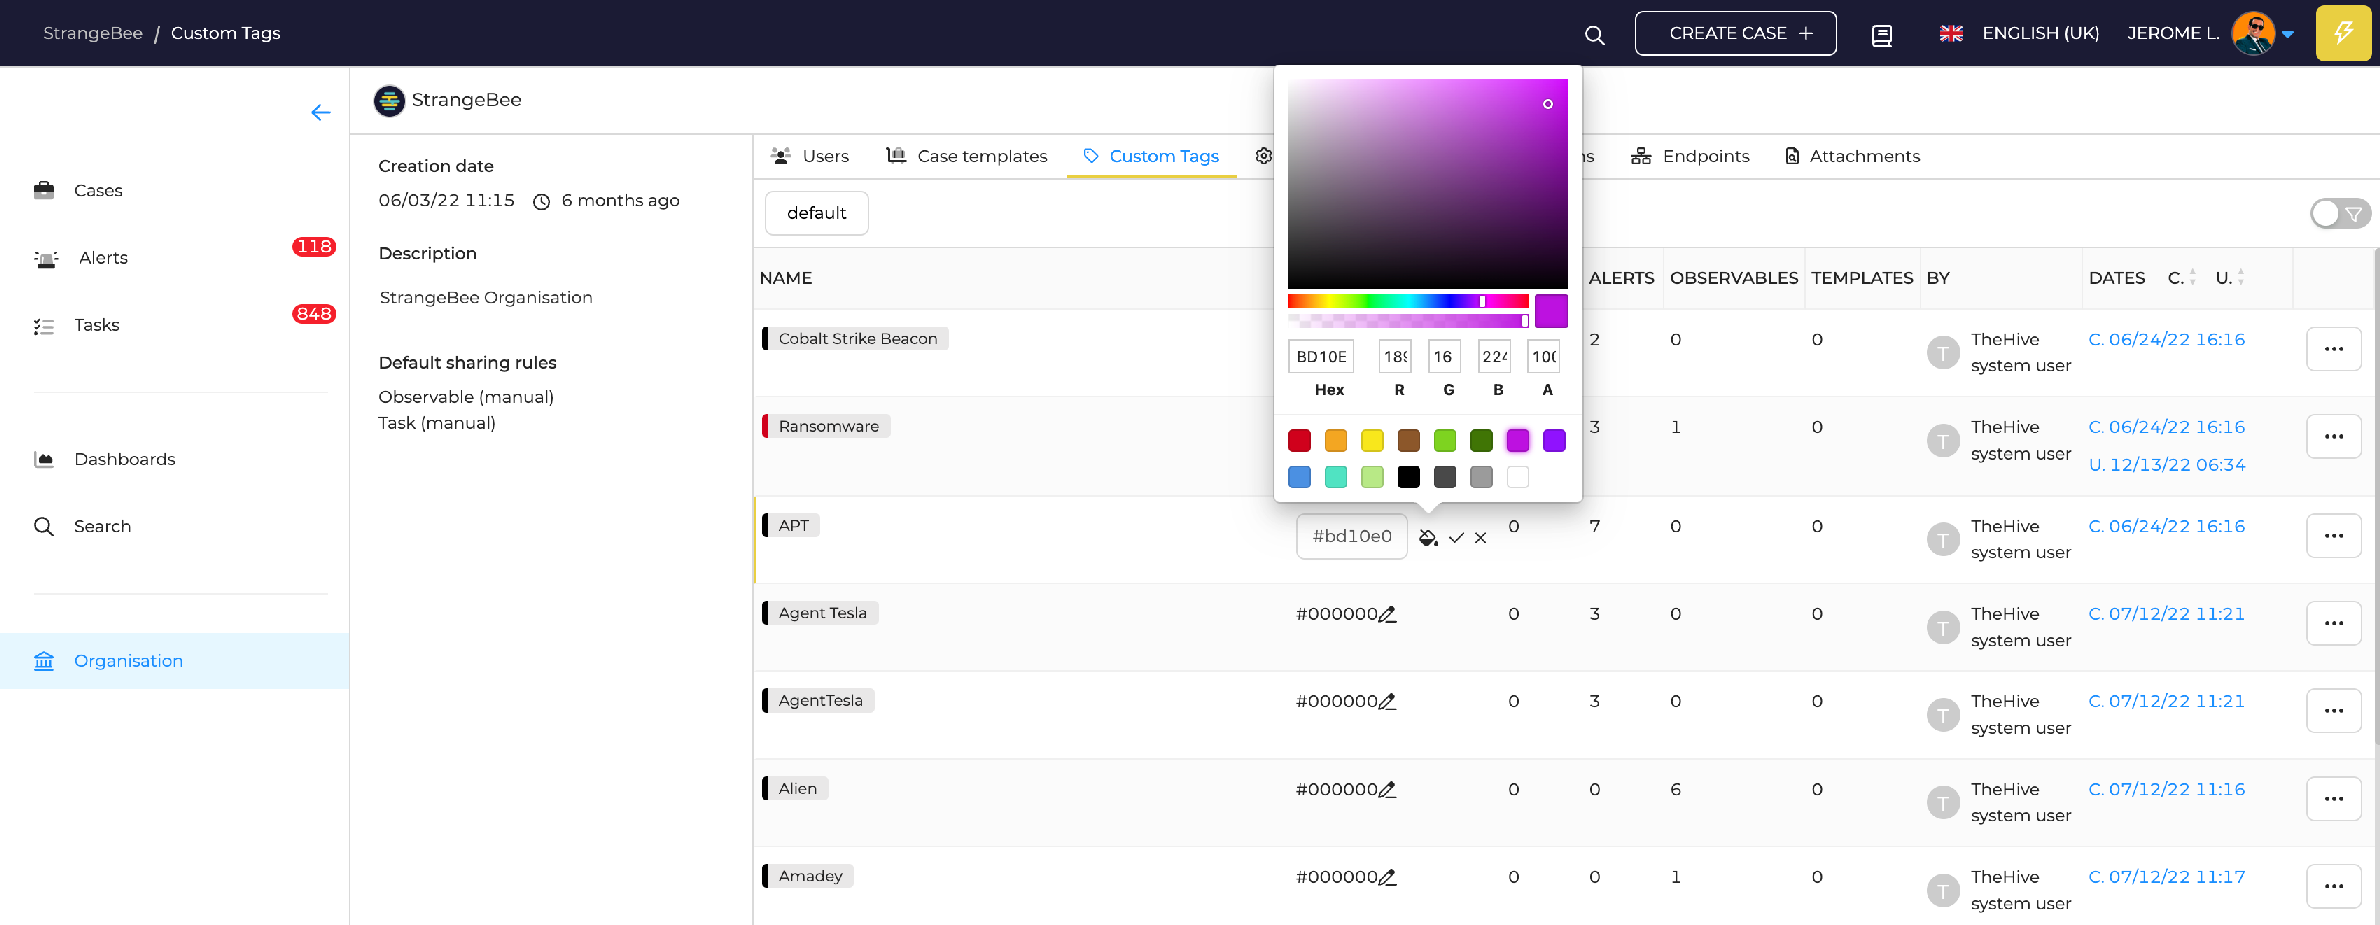
\includegraphics[width=468.01pt,height=181.9733pt]{latexImage_c391a6da51712c1e3eb1a16f82c12af7.png}}
\put(241.74,-335.432){\fontsize{9.9626}{1}\usefont{T1}{cmr}{m}{n}\selectfont\color{color_29791}Figure 8: Custom tags}
\put(56.99998,-368.906){\fontsize{9.9626}{1}\usefont{T1}{cmr}{b}{n}\selectfont\color{color_29791}Configuration}
\put(71.94498,-386.839){\fontsize{9.9626}{1}\usefont{T1}{cmr}{m}{n}\selectfont\color{color_29791}• Names and colors can be adjusted for all Custom tags}
\put(71.94498,-398.794){\fontsize{9.9626}{1}\usefont{T1}{cmr}{m}{n}\selectfont\color{color_29791}• Each tag can also be deleted}
\put(56.99998,-416.727){\fontsize{9.9626}{1}\usefont{T1}{cmr}{m}{n}\selectfont\color{color_29791}Warning: Deleting a tag from this menu will remove the tag on every Alert, Case and Observables in the}
\put(56.99998,-428.682){\fontsize{9.9626}{1}\usefont{T1}{cmr}{m}{n}\selectfont\color{color_29791}organisation.!}
\end{picture}
\begin{tikzpicture}[overlay]
\path(0pt,0pt);
\draw[color_29791,line width=0.996pt]
(57pt, -727.435pt) -- (525pt, -727.435pt)
;
\end{tikzpicture}
\begin{picture}(-5,0)(2.5,0)
\put(514.041,-739.888){\fontsize{9.9626}{1}\usefont{T1}{cmr}{b}{n}\selectfont\color{color_29791}14}
\end{picture}
\newpage

\begin{picture}(-5,0)(2.5,0)
\put(57,-71.96301){\fontsize{11.9552}{1}\usefont{T1}{cmr}{b}{n}\selectfont\color{color_29791}5.2 Analyst}
\put(57,-90.35199){\fontsize{9.9626}{1}\usefont{T1}{cmr}{b}{n}\selectfont\color{color_29791}5.2.1 Cases}
\put(71.945,-108.741){\fontsize{9.9626}{1}\usefont{T1}{cmr}{m}{n}\selectfont\color{color_29791}• Create}
\put(81.907,-134.637){\fontsize{9.9626}{1}\usefont{T1}{cmr}{b}{n}\selectfont\color{color_29791}Create new cases}
\put(81.907,-152.5699){\fontsize{9.9626}{1}\usefont{T1}{cmr}{m}{n}\selectfont\color{color_29791}A  User can create new cases using templates. Click Create Case + on the header}
\put(57,-214.733){
\includegraphics[width=468.0209pt,height=47.27484pt]{latexImage_1132a3d85233c59742de31354f61b870.png}}
\put(229.564,-233.064){\fontsize{9.9626}{1}\usefont{T1}{cmr}{m}{n}\selectfont\color{color_29791}Figure 9: create case header}
\put(81.907,-266.539){\fontsize{9.9626}{1}\usefont{T1}{cmr}{m}{n}\selectfont\color{color_29791}A new screen opens. A user can create cases by selecting any one of the following options:}
\put(81.907,-284.472){\fontsize{9.9626}{1}\usefont{T1}{cmr}{m}{n}\selectfont\color{color_29791}Click the below links to create each type of new case.}
\put(81.907,-302.404){\fontsize{9.9626}{1}\usefont{T1}{cmr}{m}{n}\selectfont\color{color_29791}Empty Case EDR / Phishing Template Archive MISP}
\put(103.799,-670.551){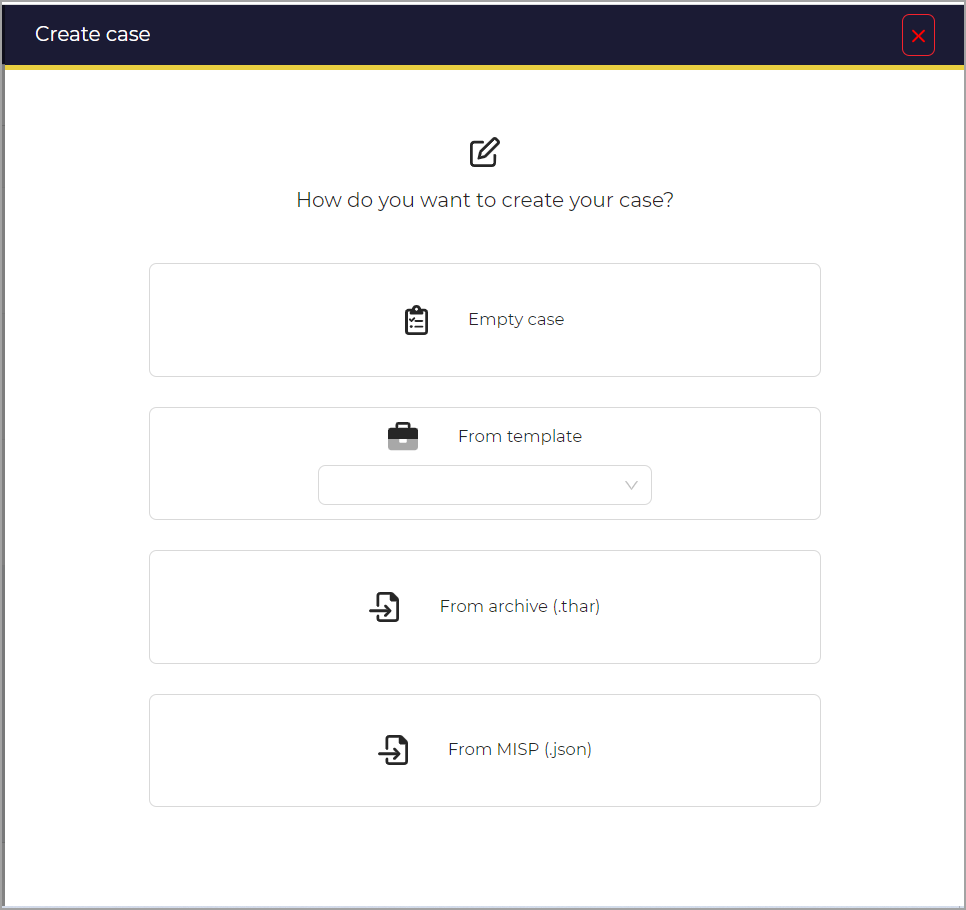
\includegraphics[width=374.41pt,height=352.7051pt]{latexImage_b3baa0d57438cda7a3cf8c269903ab93.png}}
\put(243.138,-688.882){\fontsize{9.9626}{1}\usefont{T1}{cmr}{m}{n}\selectfont\color{color_29791}Figure 10: create case}
\end{picture}
\begin{tikzpicture}[overlay]
\path(0pt,0pt);
\draw[color_29791,line width=0.996pt]
(57pt, -727.435pt) -- (525pt, -727.435pt)
;
\end{tikzpicture}
\begin{picture}(-5,0)(2.5,0)

\put(514.041,-739.888){\fontsize{9.9626}{1}\usefont{T1}{cmr}{b}{n}\selectfont\color{color_29791}15}
\end{picture}
\newpage

\begin{picture}(-5,0)(2.5,0)
\put(81.907,-71.96301){\fontsize{9.9626}{1}\usefont{T1}{cmr}{b}{n}\selectfont\color{color_29791}From an empty case}
\put(81.907,-89.89502){\fontsize{9.9626}{1}\usefont{T1}{cmr}{m}{n}\selectfont\color{color_29791}Create a new case from an empty case.}
\put(93.115,-107.828){\fontsize{9.9626}{1}\usefont{T1}{cmr}{b}{n}\selectfont\color{color_29791}– Enter the case title in the Title.}
\put(93.115,-119.783){\fontsize{9.9626}{1}\usefont{T1}{cmr}{b}{n}\selectfont\color{color_29791}– Select the date from the Date.}
\put(93.115,-131.738){\fontsize{9.9626}{1}\usefont{T1}{cmr}{b}{n}\selectfont\color{color_29791}– Select Severity,(Low/Medium/High/Critical).}
\put(93.115,-143.694){\fontsize{9.9626}{1}\usefont{T1}{cmr}{b}{n}\selectfont\color{color_29791}– Select TLP , (White/Green/Amber/Red).}
\put(93.115,-155.649){\fontsize{9.9626}{1}\usefont{T1}{cmr}{b}{n}\selectfont\color{color_29791}– Select PAP , (White/Green/Am b er/Red).}
\put(93.115,-167.6041){\fontsize{9.9626}{1}\usefont{T1}{cmr}{b}{n}\selectfont\color{color_29791}– Click + to add Tags. (Refer to Add tags).}
\put(93.115,-179.5591){\fontsize{9.9626}{1}\usefont{T1}{cmr}{b}{n}\selectfont\color{color_29791}– Enter the case description in the Description.}
\put(93.115,-191.5141){\fontsize{9.9626}{1}\usefont{T1}{cmr}{b}{n}\selectfont\color{color_29791}– Choose a Task rule from the list, (manual/existingOnly/upcommingOnly/all).}
\put(93.115,-203.4701){\fontsize{9.9626}{1}\usefont{T1}{cmr}{b}{n}\selectfont\color{color_29791}– Choose an Observable rule from the list, (manual/existingOnly/upcommingOnly/all).}
\put(93.115,-215.4251){\fontsize{9.9626}{1}\usefont{T1}{cmr}{b}{n}\selectfont\color{color_29791}– Add Tasks. (Refer to Add tasks).}
\put(93.115,-227.3801){\fontsize{9.9626}{1}\usefont{T1}{cmr}{b}{n}\selectfont\color{color_29791}– Add Custom Fields. (Refer to Add custom field values).}
\put(93.115,-239.3351){\fontsize{9.9626}{1}\usefont{T1}{cmr}{b}{n}\selectfont\color{color_29791}–}
\put(127.201,-683.86){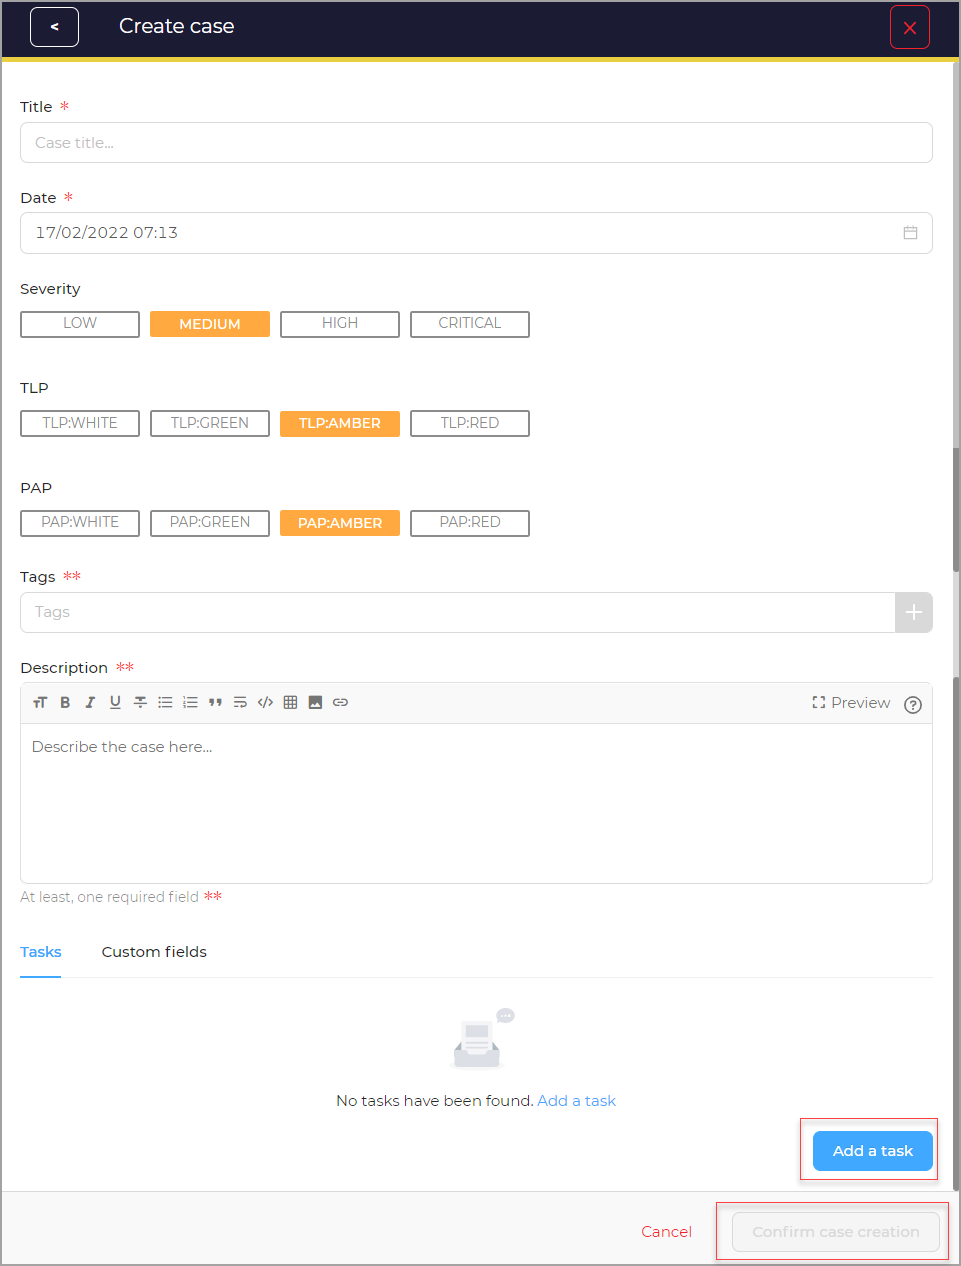
\includegraphics[width=327.6011pt,height=431.5743pt]{latexImage_52cb271ba61727c96751c573f69ce2d3.png}}
\put(227.917,-702.192){\fontsize{9.9626}{1}\usefont{T1}{cmr}{m}{n}\selectfont\color{color_29791}Figure 11: create empty case}
\end{picture}
\begin{tikzpicture}[overlay]
\path(0pt,0pt);
\draw[color_29791,line width=0.996pt]
(57pt, -727.435pt) -- (525pt, -727.435pt)
;
\end{tikzpicture}
\begin{picture}(-5,0)(2.5,0)
\put(514.041,-739.888){\fontsize{9.9626}{1}\usefont{T1}{cmr}{b}{n}\selectfont\color{color_29791}16}
\end{picture}
\newpage
\begin{picture}(-5,0)(2.5,0)
\put(81.907,-71.96301){\fontsize{9.9626}{1}\usefont{T1}{cmr}{b}{n}\selectfont\color{color_29791}From template}
\put(93.115,-89.89502){\fontsize{9.9626}{1}\usefont{T1}{cmr}{b}{n}\selectfont\color{color_29791}– Enter the case title in the Title.}
\put(93.115,-101.851){\fontsize{9.9626}{1}\usefont{T1}{cmr}{b}{n}\selectfont\color{color_29791}– Select the date from the Date.}
\put(93.115,-113.806){\fontsize{9.9626}{1}\usefont{T1}{cmr}{b}{n}\selectfont\color{color_29791}– Select Severity , (Low/Medium/High/Critical).}
\put(93.115,-125.761){\fontsize{9.9626}{1}\usefont{T1}{cmr}{b}{n}\selectfont\color{color_29791}– Select TLP , (White/Green/Amber/Red).}
\put(93.115,-137.7161){\fontsize{9.9626}{1}\usefont{T1}{cmr}{b}{n}\selectfont\color{color_29791}– Select PAP , (White/Green/Amber/Red).}
\put(93.115,-149.6711){\fontsize{9.9626}{1}\usefont{T1}{cmr}{b}{n}\selectfont\color{color_29791}– Click + to add Tags. (Refer to Add tags.)}
\put(93.115,-161.6261){\fontsize{9.9626}{1}\usefont{T1}{cmr}{b}{n}\selectfont\color{color_29791}– Enter the case description in the Description.}
\put(93.115,-173.5821){\fontsize{9.9626}{1}\usefont{T1}{cmr}{b}{n}\selectfont\color{color_29791}– Choose a T ask rule from the list, (manual/existingOnly/upcommingOnly/all).}
\put(93.115,-185.5371){\fontsize{9.9626}{1}\usefont{T1}{cmr}{b}{n}\selectfont\color{color_29791}– Choose an Observable rule from the list, (manual/existingOnly/upcommingOnly/all).}
\put(93.115,-197.4921){\fontsize{9.9626}{1}\usefont{T1}{cmr}{b}{n}\selectfont\color{color_29791}– Add Tasks. (Refer to Add tasks. / Edit tasks. /Delete tasks.)}
\put(93.115,-209.4471){\fontsize{9.9626}{1}\usefont{T1}{cmr}{b}{n}\selectfont\color{color_29791}– Add Custom Fields. (Refer to Add custom field values. /Edit custom field values. /Delete custom}
\put(103.824,-221.4022){\fontsize{9.9626}{1}\usefont{T1}{cmr}{m}{n}\selectfont\color{color_29791}field values.)}
\put(93.115,-233.3572){\fontsize{9.9626}{1}\usefont{T1}{cmr}{b}{n}\selectfont\color{color_29791}– Add Pages. (Refer to Add pages. /Delete pages.) Sharing ( Refer to Sharing.)}
\put(93.115,-245.3132){\fontsize{9.9626}{1}\usefont{T1}{cmr}{b}{n}\selectfont\color{color_29791}–}
\put(103.799,-654.632){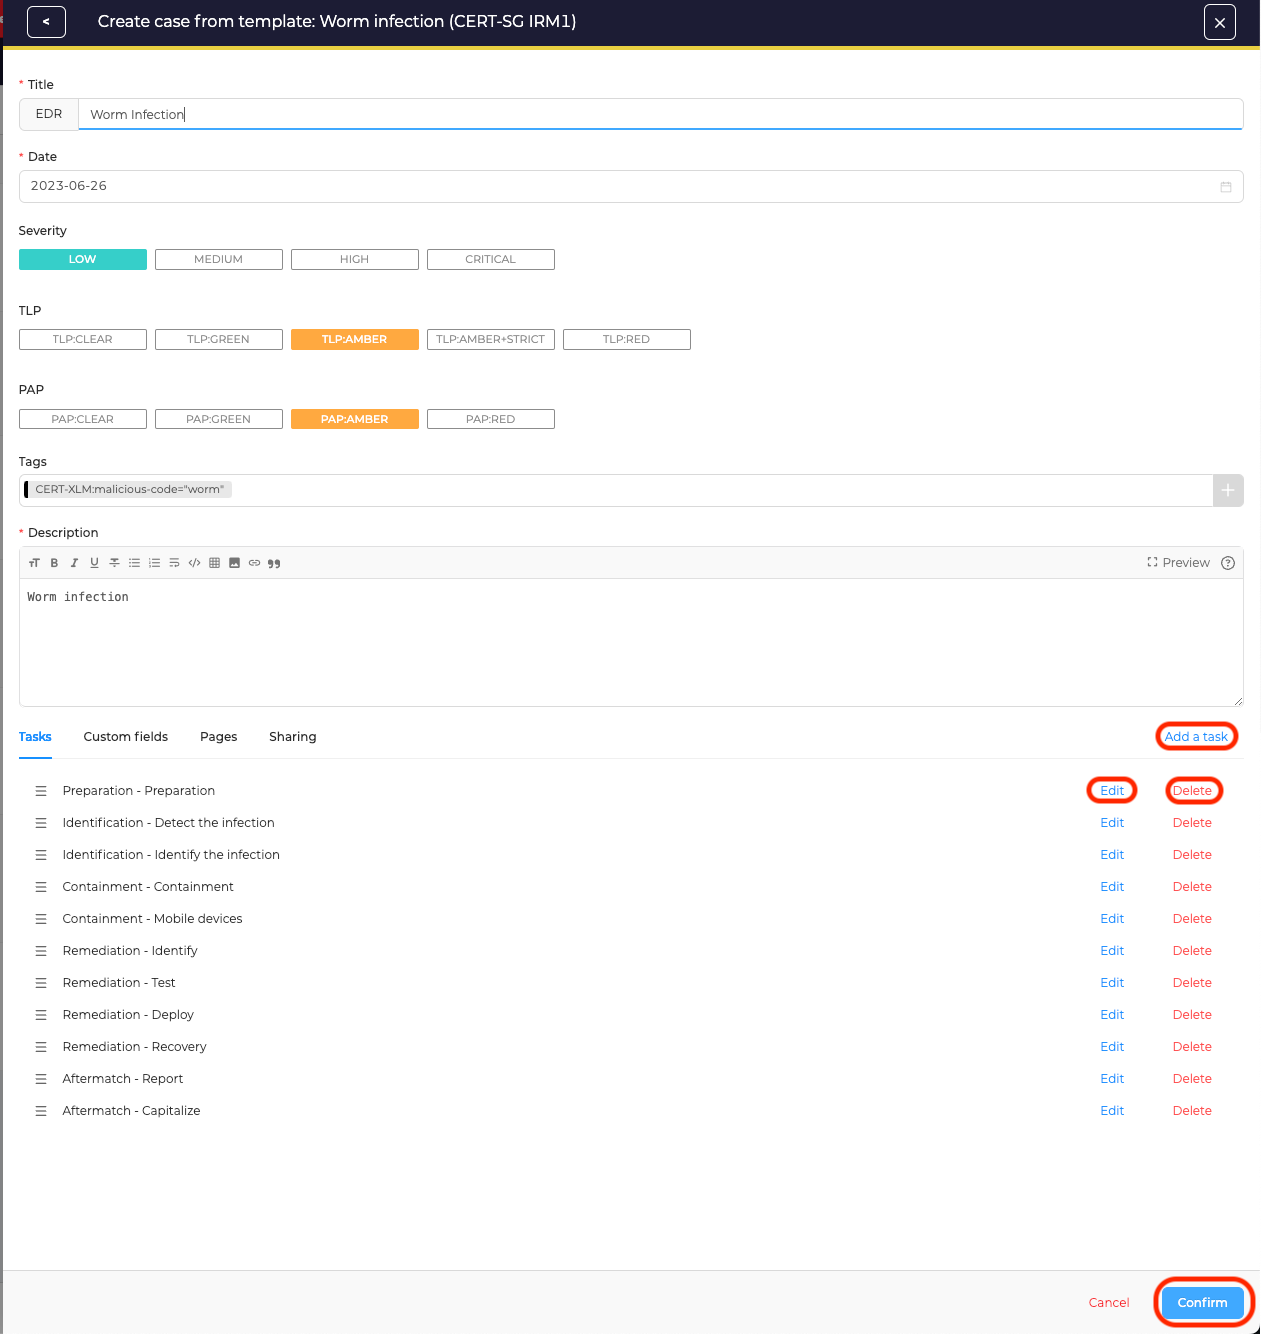
\includegraphics[width=374.3909pt,height=396.3615pt]{latexImage_b129024c5538a63ee2b55f35f8bdb8b6.png}}
\put(210.607,-672.963){\fontsize{9.9626}{1}\usefont{T1}{cmr}{m}{n}\selectfont\color{color_29791}Figure 12: create case from template}
\end{picture}
\begin{tikzpicture}[overlay]
\path(0pt,0pt);
\draw[color_29791,line width=0.996pt]
(57pt, -727.435pt) -- (525pt, -727.435pt)
;
\end{tikzpicture}
\begin{picture}(-5,0)(2.5,0)
\put(514.041,-739.888){\fontsize{9.9626}{1}\usefont{T1}{cmr}{b}{n}\selectfont\color{color_29791}17}
\end{picture}
\newpage
\begin{picture}(-5,0)(2.5,0)
\put(71.945,-71.96301){\fontsize{9.9626}{1}\usefont{T1}{cmr}{m}{n}\selectfont\color{color_29791}• Preview}
\put(81.907,-97.85901){\fontsize{9.9626}{1}\usefont{T1}{cmr}{b}{n}\selectfont\color{color_29791}Preview Cases}
\put(81.907,-115.791){\fontsize{9.9626}{1}\usefont{T1}{cmr}{m}{n}\selectfont\color{color_29791}On the list of case details page, there is a Preview button corresponding to the specific case name.}
\put(81.907,-127.746){\fontsize{9.9626}{1}\usefont{T1}{cmr}{m}{n}\selectfont\color{color_29791}Click the Preview option}
\put(57,-249.975){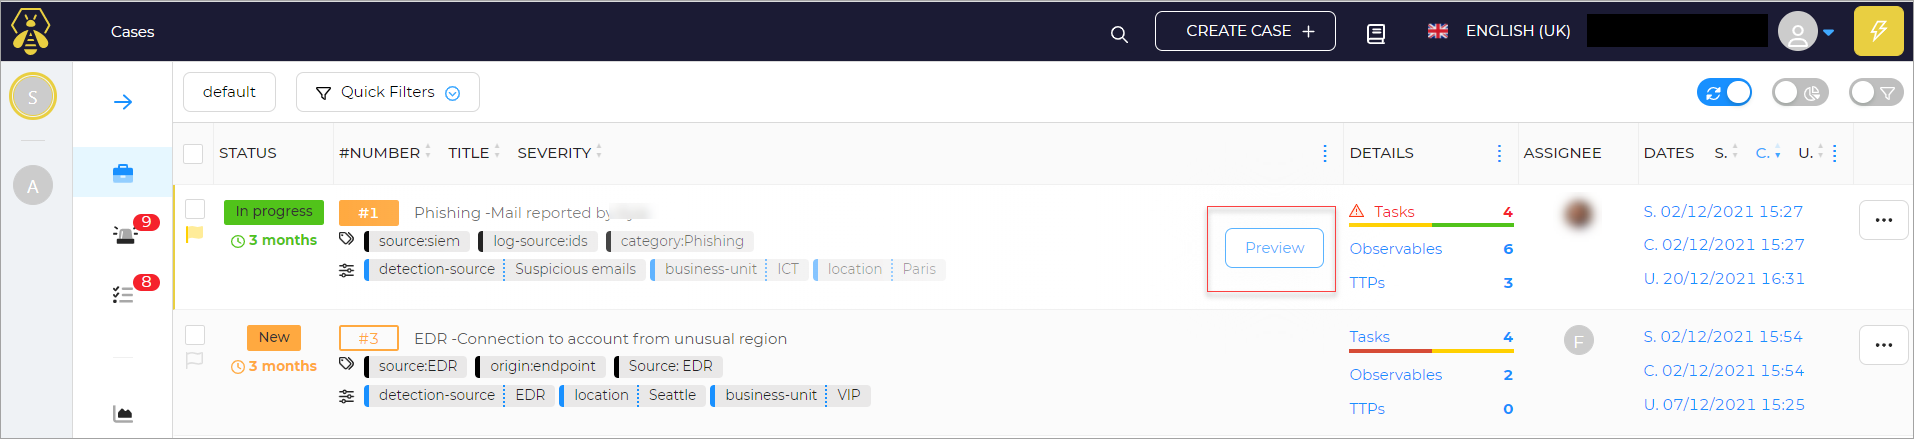
\includegraphics[width=467.9959pt,height=107.3408pt]{latexImage_e3773f8056660f380760c1efe2f0d3dd.png}}
\put(249.489,-268.306){\fontsize{9.9626}{1}\usefont{T1}{cmr}{m}{n}\selectfont\color{color_29791}Figure 13: case list}
\put(81.90701,-301.78){\fontsize{9.9626}{1}\usefont{T1}{cmr}{m}{n}\selectfont\color{color_29791}The case details preview window opens.}

\put(57,-705.86){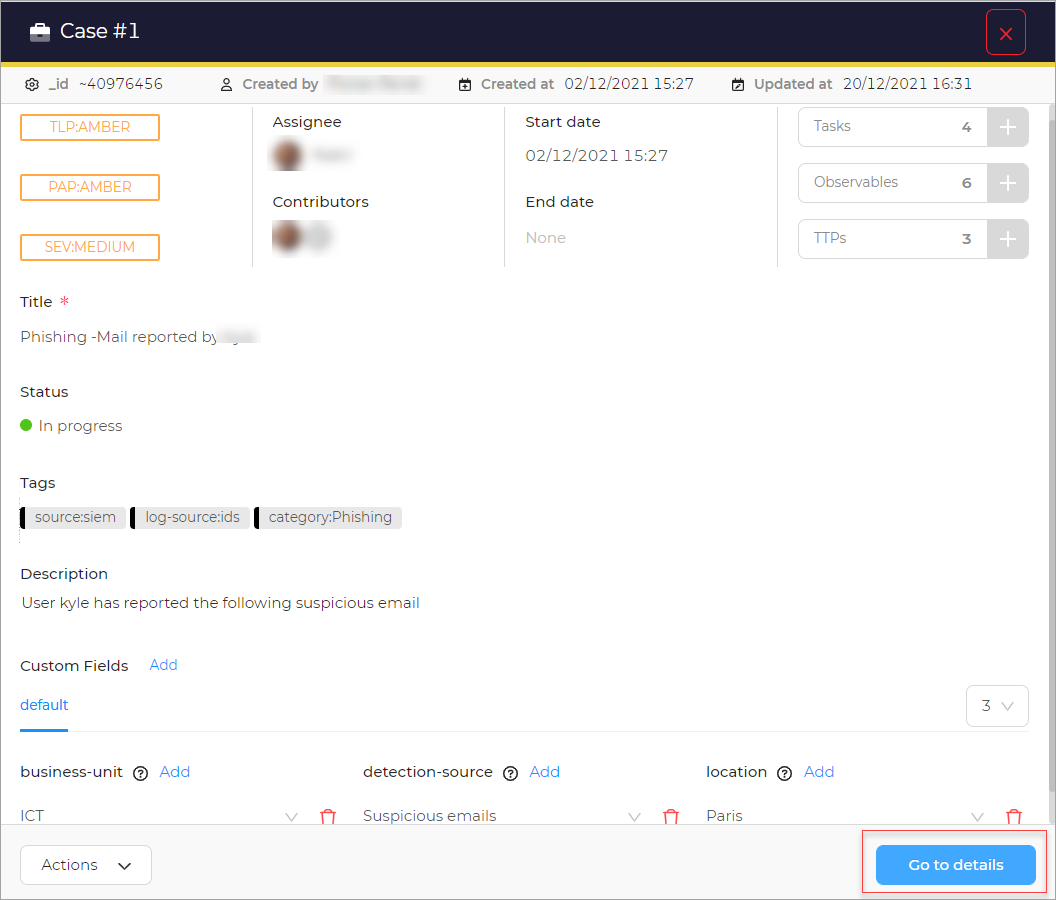
\includegraphics[width=467.996pt,height=398.8602pt]{latexImage_eba70116e4703513f9fc681c186ebc6a.png}}

\end{picture}
\begin{tikzpicture}[overlay]
\path(0pt,0pt);
\draw[color_29791,line width=0.996pt]
(57pt, -727.435pt) -- (525pt, -727.435pt)
;
\end{tikzpicture}
\begin{picture}(-5,0)(2.5,0)
\put(514.041,-739.888){\fontsize{9.9626}{1}\usefont{T1}{cmr}{b}{n}\selectfont\color{color_29791}18}
\end{picture}
\newpage
\begin{picture}(-5,0)(2.5,0)
\put(71.945,-71.96301){\fontsize{9.9626}{1}\usefont{T1}{cmr}{m}{n}\selectfont\color{color_29791}• Adding Task and Pages}
\put(81.907,-97.85901){\fontsize{9.9626}{1}\usefont{T1}{cmr}{b}{n}\selectfont\color{color_29791}Add tasks}
\put(81.907,-115.791){\fontsize{9.9626}{1}\usefont{T1}{cmr}{m}{n}\selectfont\color{color_29791}The task Group is default.}
\put(93.115,-133.724){\fontsize{9.9626}{1}\usefont{T1}{cmr}{b}{n}\selectfont\color{color_29791}– Enter the task Title.}
\put(93.115,-145.679){\fontsize{9.9626}{1}\usefont{T1}{cmr}{b}{n}\selectfont\color{color_29791}– Enter the task description in the Description.}
\put(93.115,-157.634){\fontsize{9.9626}{1}\usefont{T1}{cmr}{b}{n}\selectfont\color{color_29791}– Switch the toggle button to Flag this task?.}
\put(93.115,-169.59){\fontsize{9.9626}{1}\usefont{T1}{cmr}{b}{n}\selectfont\color{color_29791}– Select the Due date.}
\put(93.115,-181.545){\fontsize{9.9626}{1}\usefont{T1}{cmr}{b}{n}\selectfont\color{color_29791}– Click Save and add another, to add another task.}
\put(93.115,-193.5001){\fontsize{9.9626}{1}\usefont{T1}{cmr}{b}{n}\selectfont\color{color_29791}–}
\put(103.799,-596.434){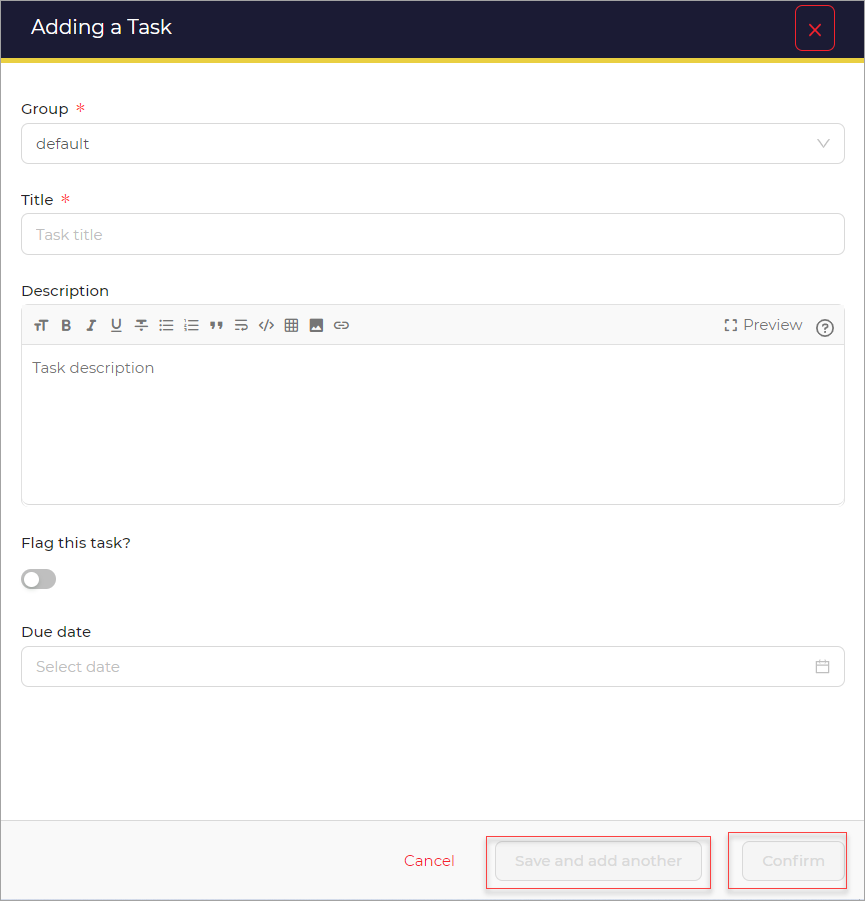
\includegraphics[width=374.4014pt,height=389.9834pt]{latexImage_6d16249b18f67b449411461eaeb6d8af.png}}
\put(243.843,-614.765){\fontsize{9.9626}{1}\usefont{T1}{cmr}{m}{n}\selectfont\color{color_29791}Figure 14: add a task}
\put(81.90698,-648.239){\fontsize{9.9626}{1}\usefont{T1}{cmr}{b}{n}\selectfont\color{color_29791}Add tags}
\put(81.90698,-666.172){\fontsize{9.9626}{1}\usefont{T1}{cmr}{m}{n}\selectfont\color{color_29791}Choose tags from the Taxonomy . The selected tag will appear in the Selected Tags box. Click the Add}
\put(81.90698,-678.127){\fontsize{9.9626}{1}\usefont{T1}{cmr}{m}{n}\selectfont\color{color_29791}selected tags button.}
\end{picture}
\begin{tikzpicture}[overlay]
\path(0pt,0pt);
\draw[color_29791,line width=0.996pt]
(57pt, -727.435pt) -- (525pt, -727.435pt)
;
\end{tikzpicture}
\begin{picture}(-5,0)(2.5,0)
\put(514.041,-739.888){\fontsize{9.9626}{1}\usefont{T1}{cmr}{b}{n}\selectfont\color{color_29791}19}
\end{picture}
\newpage
\begin{picture}(-5,0)(2.5,0)
\put(127.201,-404.808){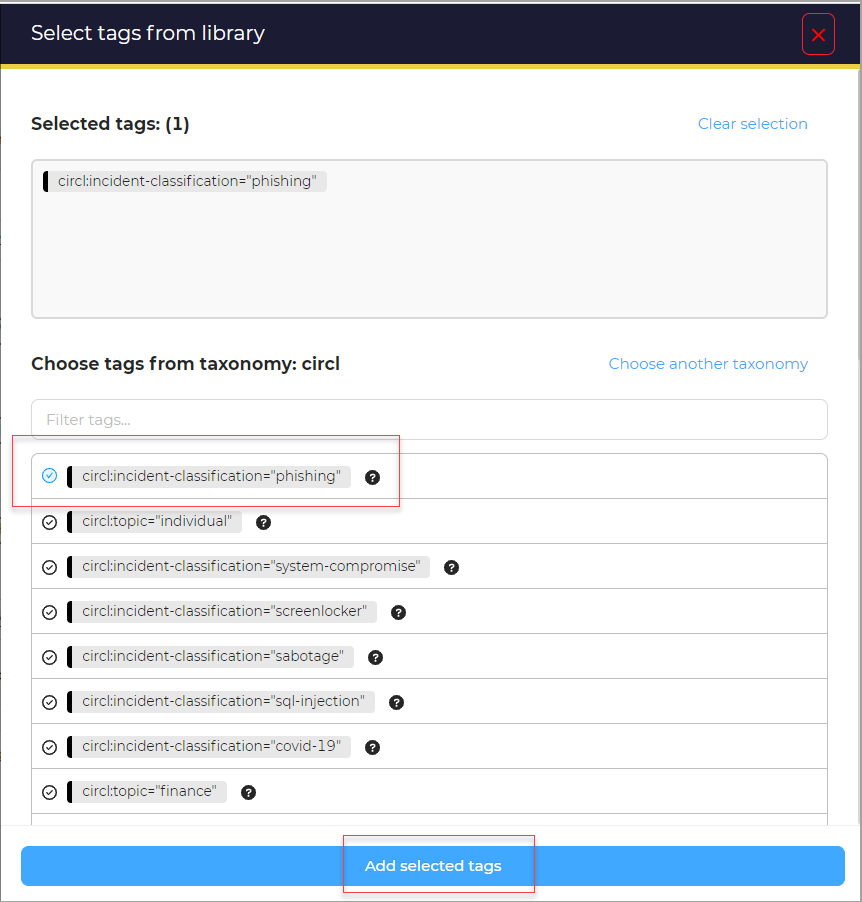
\includegraphics[width=327.6048pt,height=342.8069pt]{latexImage_64791aba64ea59f36988e0d35baa659a.png}}
\put(248.133,-423.139){\fontsize{9.9626}{1}\usefont{T1}{cmr}{m}{n}\selectfont\color{color_29791}Figure 15: add tags}
\put(81.907,-456.613){\fontsize{9.9626}{1}\usefont{T1}{cmr}{b}{n}\selectfont\color{color_29791}Add pages}
\put(81.907,-474.546){\fontsize{9.9626}{1}\usefont{T1}{cmr}{m}{n}\selectfont\color{color_29791}By selecting Create new page}
\put(93.115,-492.479){\fontsize{9.9626}{1}\usefont{T1}{cmr}{b}{n}\selectfont\color{color_29791}– Enter the page Title.}
\put(93.115,-504.434){\fontsize{9.9626}{1}\usefont{T1}{cmr}{b}{n}\selectfont\color{color_29791}– Enter or select the Category .}
\put(93.115,-516.389){\fontsize{9.9626}{1}\usefont{T1}{cmr}{b}{n}\selectfont\color{color_29791}– Enter the page content in the content.}
\put(93.115,-528.344){\fontsize{9.9626}{1}\usefont{T1}{cmr}{b}{n}\selectfont\color{color_29791}– Click Confirm.}
\put(93.115,-540.3){\fontsize{9.9626}{1}\usefont{T1}{cmr}{b}{n}\selectfont\color{color_29791}– Click Save and add another, to add another task.}
\end{picture}
\begin{tikzpicture}[overlay]
\path(0pt,0pt);
\draw[color_29791,line width=0.996pt]
(57pt, -727.435pt) -- (525pt, -727.435pt)
;
\end{tikzpicture}
\begin{picture}(-5,0)(2.5,0)
\put(514.041,-739.888){\fontsize{9.9626}{1}\usefont{T1}{cmr}{b}{n}\selectfont\color{color_29791}20}
\end{picture}
\newpage
\begin{picture}(-5,0)(2.5,0)
\put(57,-613.8611){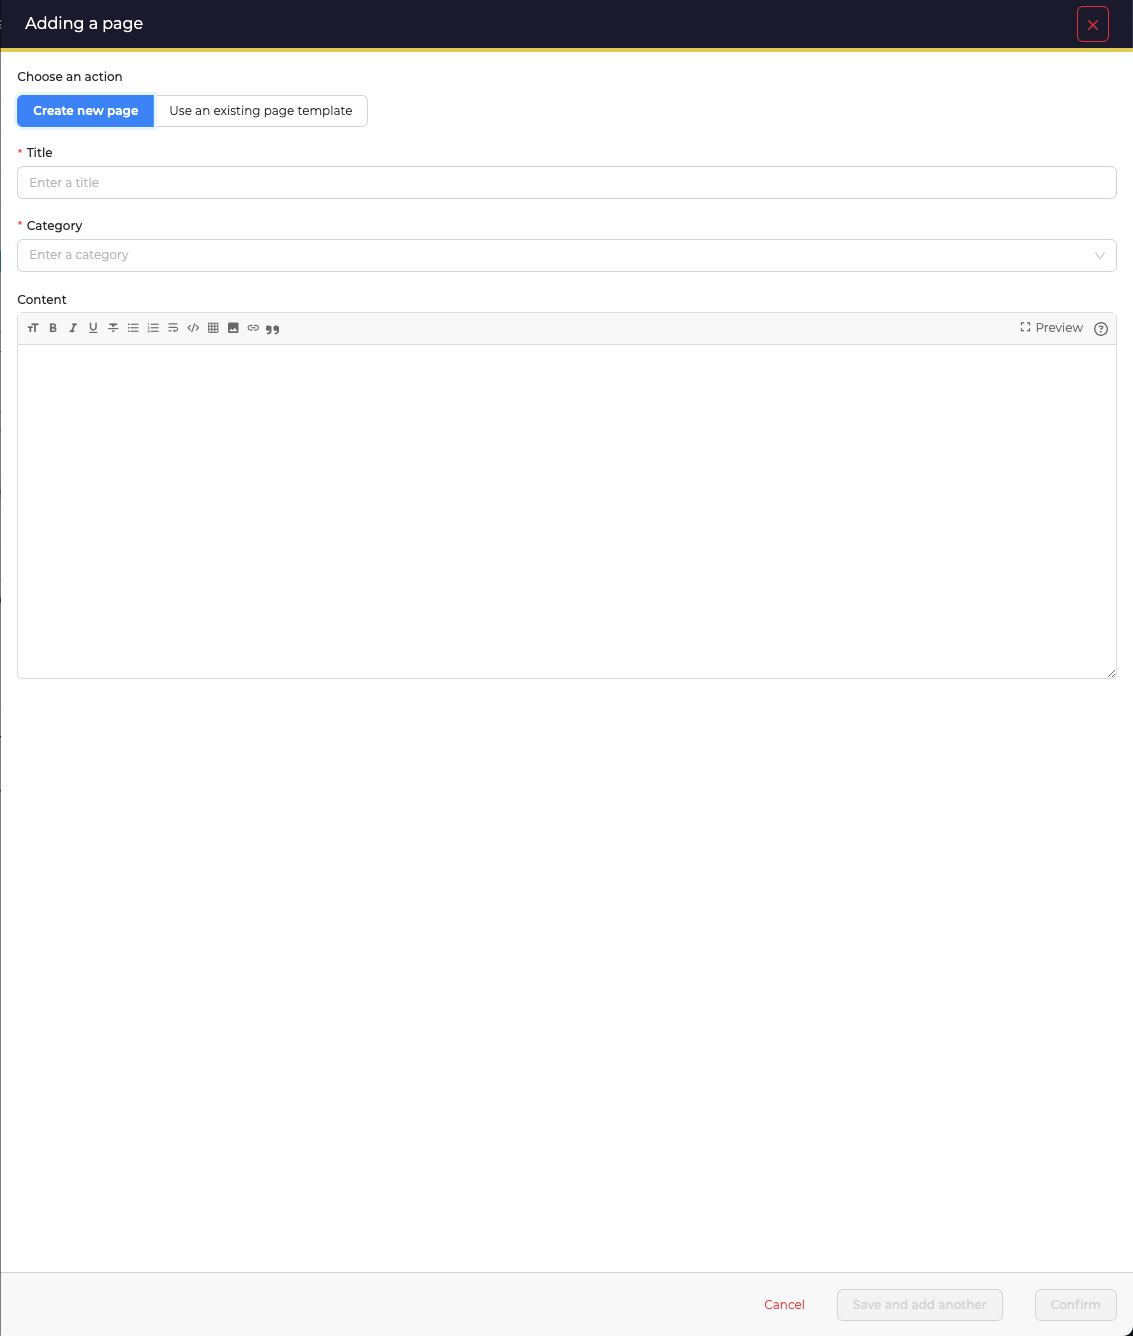
\includegraphics[width=468.0083pt,height=551.8616pt]{latexImage_f6cc5030da3686716904ba37721b3e04.png}}
\put(232.663,-632.192){\fontsize{9.9626}{1}\usefont{T1}{cmr}{m}{n}\selectfont\color{color_29791}Figure 16: add a new page}
\put(81.907,-665.667){\fontsize{9.9626}{1}\usefont{T1}{cmr}{m}{n}\selectfont\color{color_29791}By selecting Use an existing page template}
\put(81.907,-683.6){\fontsize{9.9626}{1}\usefont{T1}{cmr}{m}{n}\selectfont\color{color_29791}Choose template(s) from those available in the list of existing templates Click Confirm. Click Save and}
\put(81.907,-695.555){\fontsize{9.9626}{1}\usefont{T1}{cmr}{m}{n}\selectfont\color{color_29791}add another, to add another task.}
\end{picture}
\begin{tikzpicture}[overlay]
\path(0pt,0pt);
\draw[color_29791,line width=0.996pt]
(57pt, -727.435pt) -- (525pt, -727.435pt)
;
\end{tikzpicture}
\begin{picture}(-5,0)(2.5,0)
\put(514.041,-739.888){\fontsize{9.9626}{1}\usefont{T1}{cmr}{b}{n}\selectfont\color{color_29791}21}
\end{picture}
\newpage
\begin{picture}(-5,0)(2.5,0)
\put(103.799,-681.81){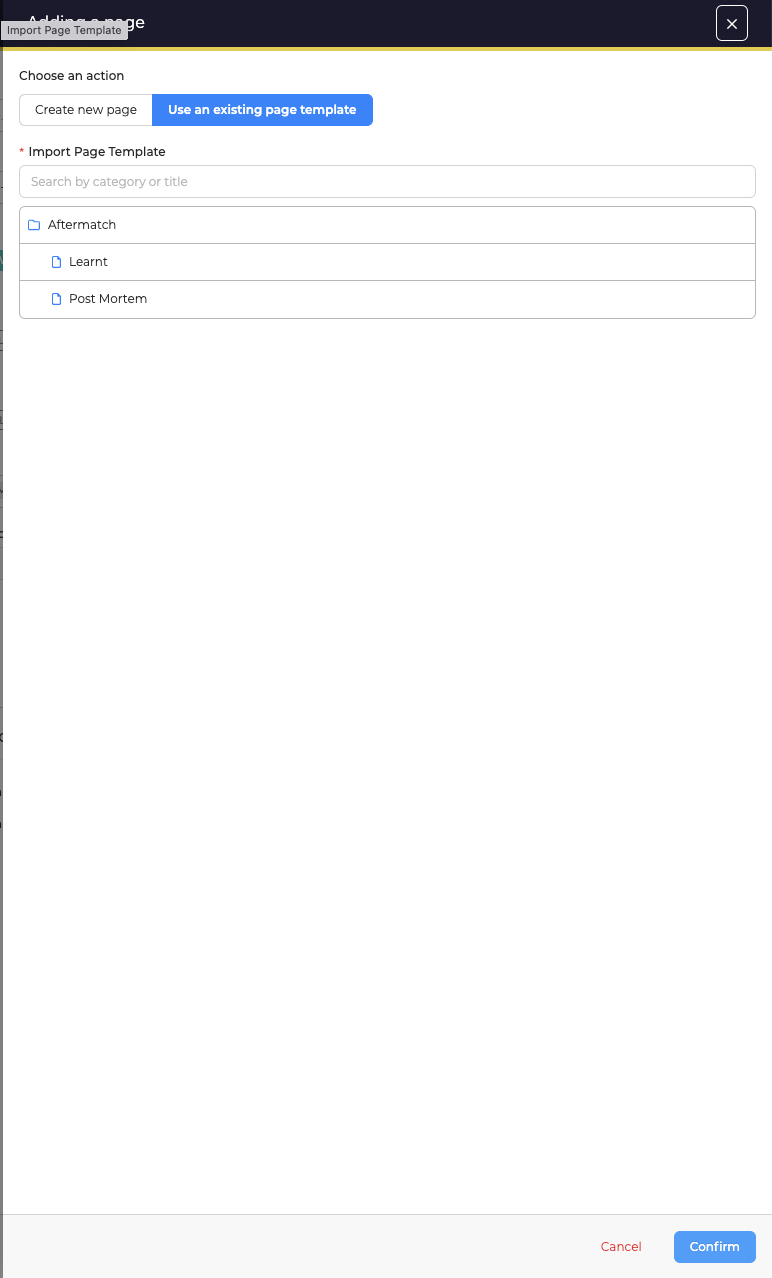
\includegraphics[width=374.4123pt,height=619.8172pt]{latexImage_c9b0661069c628db2cc8de9bdcd4a525.png}}
\put(220.044,-700.141){\fontsize{9.9626}{1}\usefont{T1}{cmr}{m}{n}\selectfont\color{color_29791}Figure 17: with an existing page}
\end{picture}
\begin{tikzpicture}[overlay]
\path(0pt,0pt);
\draw[color_29791,line width=0.996pt]
(57pt, -727.435pt) -- (525pt, -727.435pt)
;
\end{tikzpicture}
\begin{picture}(-5,0)(2.5,0)
\put(514.041,-739.888){\fontsize{9.9626}{1}\usefont{T1}{cmr}{b}{n}\selectfont\color{color_29791}22}
\end{picture}
\newpage
\begin{picture}(-5,0)(2.5,0)
\put(57,-71.96301){\fontsize{9.9626}{1}\usefont{T1}{cmr}{b}{n}\selectfont\color{color_29791}5.2.2 Tasks}
\put(71.945,-90.35199){\fontsize{9.9626}{1}\usefont{T1}{cmr}{m}{n}\selectfont\color{color_29791}• About}
\put(81.907,-116.248){\fontsize{9.9626}{1}\usefont{T1}{cmr}{b}{n}\selectfont\color{color_29791}To view task details}
\put(81.907,-134.181){\fontsize{9.9626}{1}\usefont{T1}{cmr}{m}{n}\selectfont\color{color_29791}You can click on any of the tasks in the list to view more details}
\put(57,-368.816){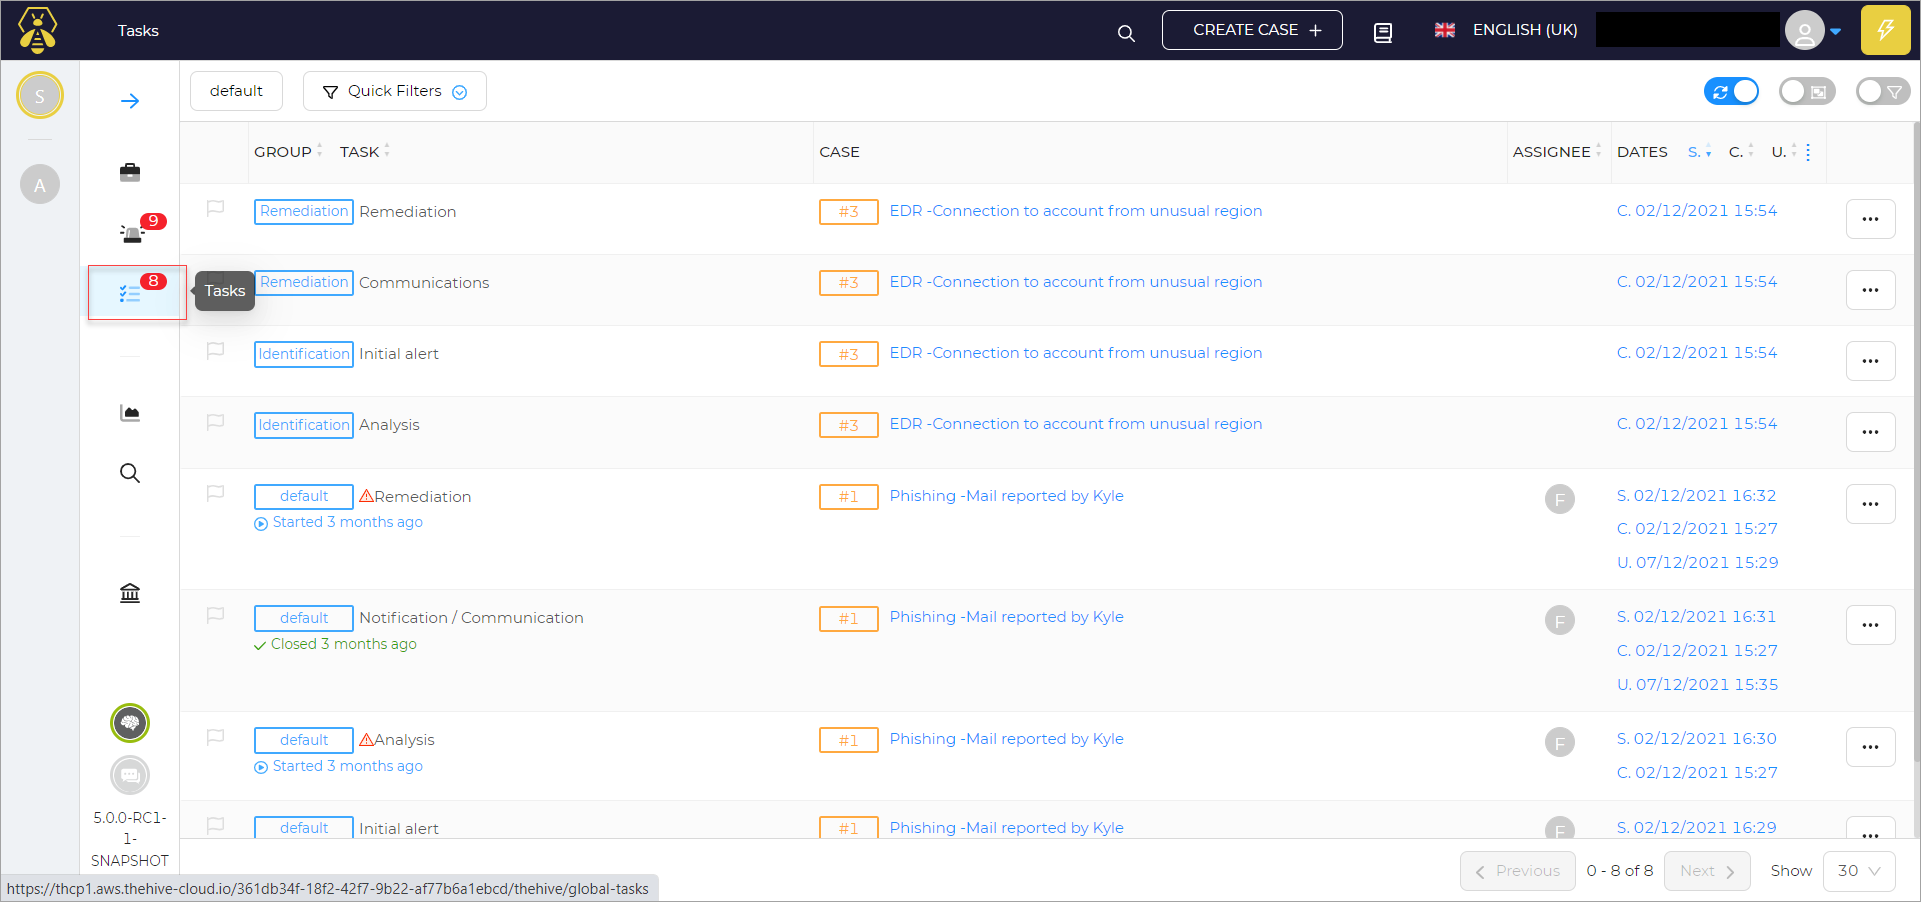
\includegraphics[width=468.0017pt,height=219.7489pt]{latexImage_8ba9cdccced3b4d1d8f690e392a85f9f.png}}
\put(249.351,-387.147){\fontsize{9.9626}{1}\usefont{T1}{cmr}{m}{n}\selectfont\color{color_29791}Figure 18: task list}
\put(81.90701,-420.621){\fontsize{9.9626}{1}\usefont{T1}{cmr}{m}{n}\selectfont\color{color_29791}The details: }
\put(57,-584.71){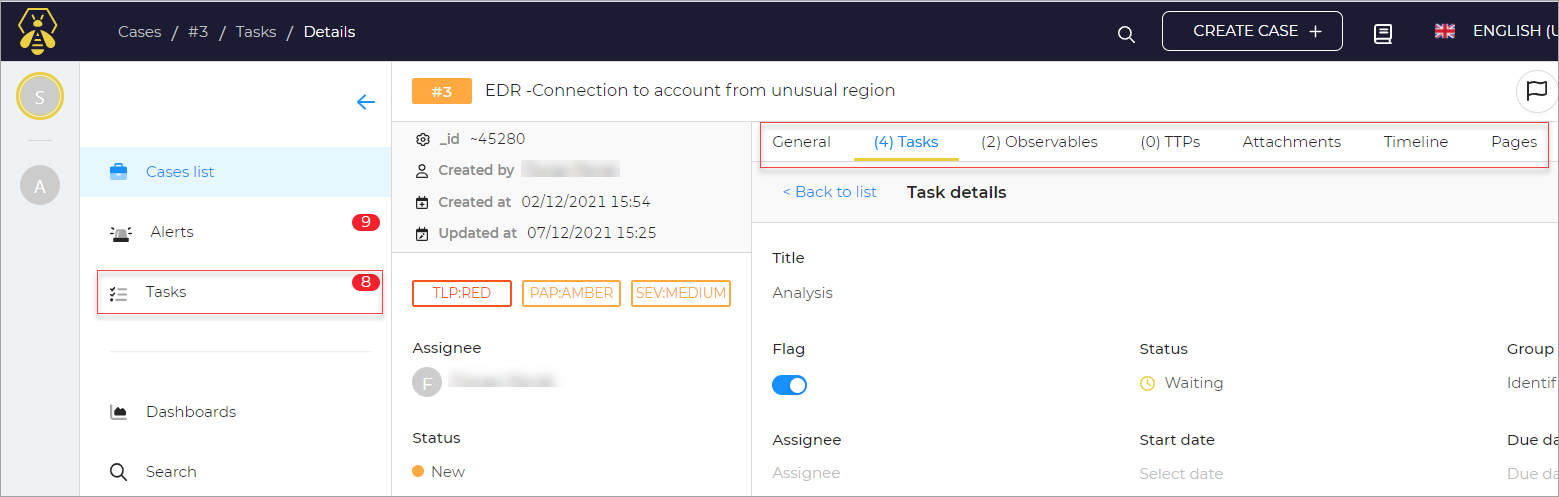
\includegraphics[width=468.018pt,height=149.2014pt]{latexImage_db1560e88309327353fa341f0d94c74f.png}}
\end{picture}
\begin{tikzpicture}[overlay]
\path(0pt,0pt);
\draw[color_29791,line width=0.996pt]
(57pt, -727.435pt) -- (525pt, -727.435pt)
;
\end{tikzpicture}
\begin{picture}(-5,0)(2.5,0)
\put(514.041,-739.888){\fontsize{9.9626}{1}\usefont{T1}{cmr}{b}{n}\selectfont\color{color_29791}23}
\end{picture}
\newpage
\begin{picture}(-5,0)(2.5,0)
\put(71.945,-71.96301){\fontsize{9.9626}{1}\usefont{T1}{cmr}{m}{n}\selectfont\color{color_29791}• Preview}
\put(81.907,-97.85901){\fontsize{9.9626}{1}\usefont{T1}{cmr}{b}{n}\selectfont\color{color_29791}To preview the task details:}
\put(81.907,-115.791){\fontsize{9.9626}{1}\usefont{T1}{cmr}{m}{n}\selectfont\color{color_29791}On the list of tasks page, there is a Preview button corresponding to the specific task name.}
\put(81.907,-133.724){\fontsize{9.9626}{1}\usefont{T1}{cmr}{m}{n}\selectfont\color{color_29791}Click the preview option}
\put(57,-291.037){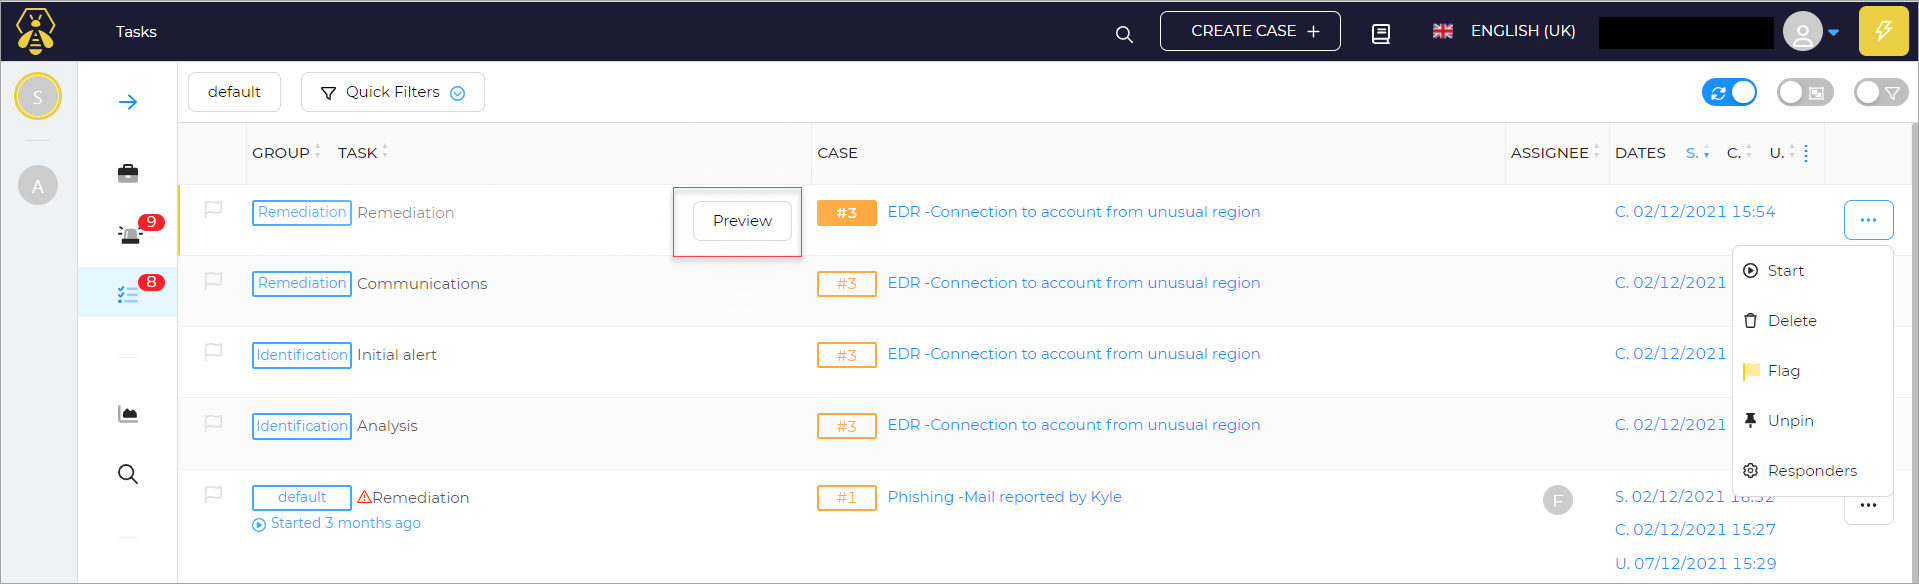
\includegraphics[width=467.998pt,height=142.4236pt]{latexImage_f43ce9104c60630e04fc936d285abc71.png}}
\put(249.351,-309.368){\fontsize{9.9626}{1}\usefont{T1}{cmr}{m}{n}\selectfont\color{color_29791}Figure 19: task list}
\put(81.90701,-342.843){\fontsize{9.9626}{1}\usefont{T1}{cmr}{m}{n}\selectfont\color{color_29791}The task details preview window opens.}
\put(57,-784.695){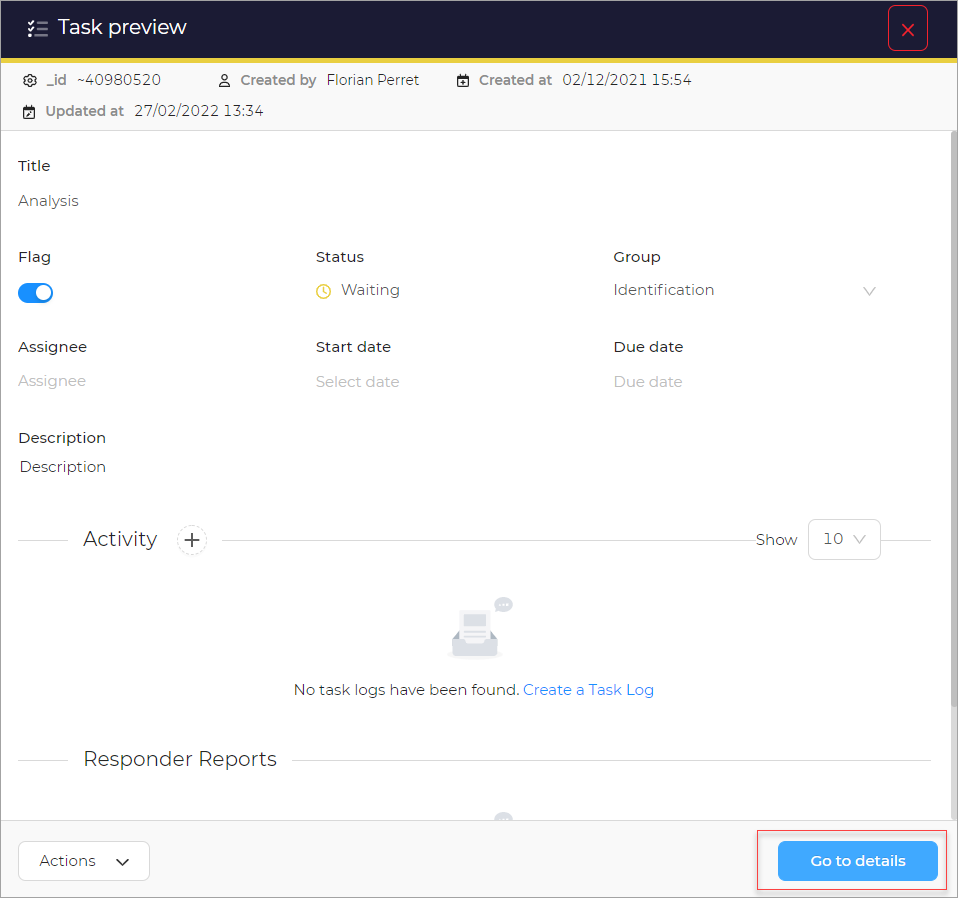
\includegraphics[width=468.0079pt,height=438.6964pt]{latexImage_cfba8b16373ea1247b4c6080fb22c1d7.png}}
\end{picture}
\newpage
\begin{picture}(-5,0)(2.5,0)
\put(71.945,-71.96301){\fontsize{9.9626}{1}\usefont{T1}{cmr}{m}{n}\selectfont\color{color_29791}• Actions}
\put(81.907,-97.85901){\fontsize{9.9626}{1}\usefont{T1}{cmr}{b}{n}\selectfont\color{color_29791}Actions}
\put(81.907,-115.791){\fontsize{9.9626}{1}\usefont{T1}{cmr}{m}{n}\selectfont\color{color_29791}You can make use of any of the available actions}
\put(57,-270.183){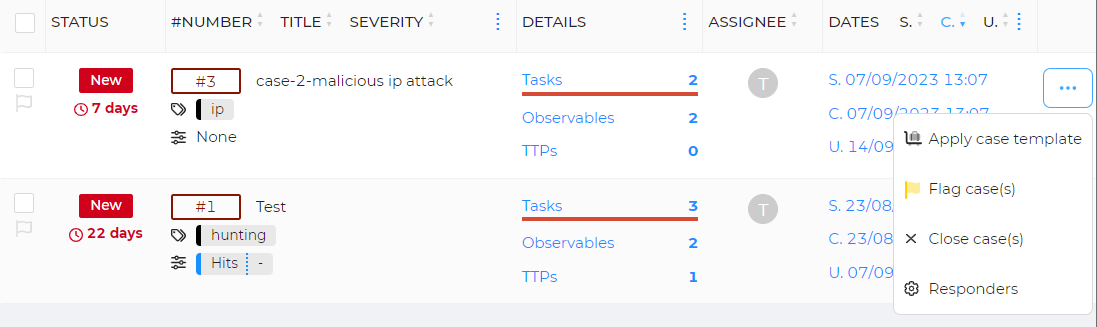
\includegraphics[width=468pt,height=139.5041pt]{latexImage_d3893852bf37fddbcdfad6b50d1d66c1.png}}
\put(81.907,-312.027){\fontsize{9.9626}{1}\usefont{T1}{cmr}{b}{n}\selectfont\color{color_29791}Flag/Unflag}
\put(81.907,-329.959){\fontsize{9.9626}{1}\usefont{T1}{cmr}{m}{n}\selectfont\color{color_29791}Click the Flag/Unflag option to either flag or unflag a case. A pop-up message appears}
\put(172.34,-395.231){
\includegraphics[width=234.004pt,height=49.82965pt]{latexImage_d646f2971df79e0b8efcb9e210c8a090.png}}
\put(81.907,-425.119){\fontsize{9.9626}{1}\usefont{T1}{cmr}{b}{n}\selectfont\color{color_29791}Close case}
\put(81.907,-443.052){\fontsize{9.9626}{1}\usefont{T1}{cmr}{m}{n}\selectfont\color{color_29791}Click the Close option to remove a case A new window opens .}
\put(93.115,-460.984){\fontsize{9.9626}{1}\usefont{T1}{cmr}{b}{n}\selectfont\color{color_29791}– Select Status from the list.}
\put(93.115,-472.939){\fontsize{9.9626}{1}\usefont{T1}{cmr}{b}{n}\selectfont\color{color_29791}– Change the Summary}
\put(93.115,-484.895){\fontsize{9.9626}{1}\usefont{T1}{cmr}{b}{n}\selectfont\color{color_29791}– Click the Close tasks and case button.}
\end{picture}
\begin{tikzpicture}[overlay]
\path(0pt,0pt);
\draw[color_29791,line width=0.996pt]
(57pt, -727.435pt) -- (525pt, -727.435pt)
;
\end{tikzpicture}
\begin{picture}(-5,0)(2.5,0)
\put(514.041,-739.888){\fontsize{9.9626}{1}\usefont{T1}{cmr}{b}{n}\selectfont\color{color_29791}25}
\end{picture}
\newpage
\begin{picture}(-5,0)(2.5,0)
\put(57,-553.334){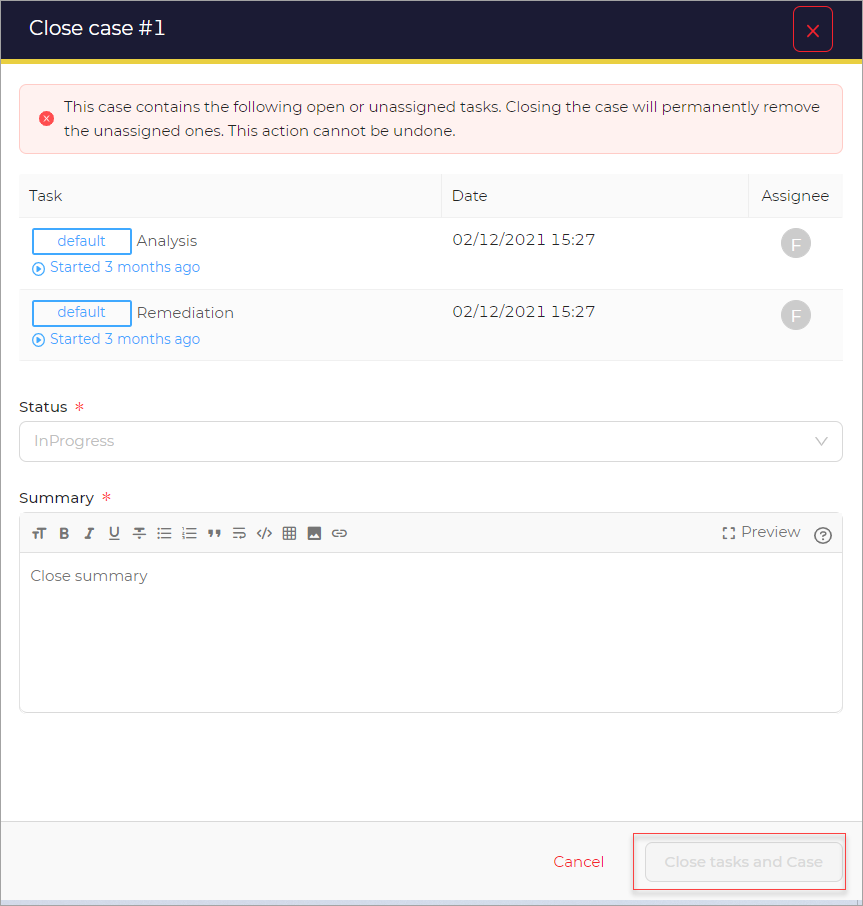
\includegraphics[width=468.0135pt,height=491.3329pt]{latexImage_d8e5d8293e1629c39de23a241bd44420.png}}
\put(235.929,-571.665){\fontsize{9.9626}{1}\usefont{T1}{cmr}{m}{n}\selectfont\color{color_29791}Figure 20: Closing a case}
\end{picture}
\begin{tikzpicture}[overlay]
\path(0pt,0pt);
\draw[color_29791,line width=0.996pt]
(57pt, -727.435pt) -- (525pt, -727.435pt)
;
\end{tikzpicture}
\begin{picture}(-5,0)(2.5,0)
\put(514.041,-739.888){\fontsize{9.9626}{1}\usefont{T1}{cmr}{b}{n}\selectfont\color{color_29791}26}
\end{picture}
\newpage
\begin{picture}(-5,0)(2.5,0)
\put(57,-71.96301){\fontsize{11.9552}{1}\usefont{T1}{cmr}{b}{n}\selectfont\color{color_29791}5.3 Observables}
\put(57,-90.35199){\fontsize{9.9626}{1}\usefont{T1}{cmr}{b}{n}\selectfont\color{color_29791}5.3.1 Create Case Observables}
\put(57,-108.741){\fontsize{9.9626}{1}\usefont{T1}{cmr}{m}{n}\selectfont\color{color_29791}In a TheHive case, observables can be declared. Open the Observables list (Case ¿ Observables) to create}
\put(57,-120.697){\fontsize{9.9626}{1}\usefont{T1}{cmr}{m}{n}\selectfont\color{color_29791}an observable. You must have permission to administer cases.}
\put(57,-138.629){\fontsize{9.9626}{1}\usefont{T1}{cmr}{m}{n}\selectfont\color{color_29791}The Add observable icon is located on the Observables tab:}
\put(57,-216.551){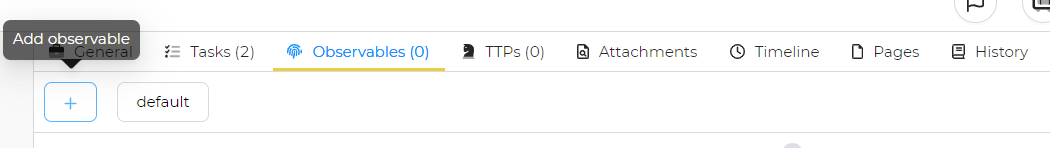
\includegraphics[width=468.0081pt,height=65.96686pt]{latexImage_02b18b02cd5a3311160933dc6673438a.png}}
\put(226.921,-234.883){\fontsize{9.9626}{1}\usefont{T1}{cmr}{m}{n}\selectfont\color{color_29791}Figure 21: Adding obserables}
\put(57,-262.38){\fontsize{9.9626}{1}\usefont{T1}{cmr}{m}{n}\selectfont\color{color_29791}In the pop-up, you are invited to fill the observable(s) details:}
\put(71.945,-280.312){\fontsize{9.9626}{1}\usefont{T1}{cmr}{m}{n}\selectfont\color{color_29791}• Type *: The observable dataType (e.g.: ip, hash, domain, ...)}
\put(71.94501,-292.268){\fontsize{9.9626}{1}\usefont{T1}{cmr}{m}{n}\selectfont\color{color_29791}• Value *: Your observable value (e.g.: 8.8.8.8)}
\put(93.11501,-304.223){\fontsize{9.9626}{1}\usefont{T1}{cmr}{b}{n}\selectfont\color{color_29791}– One observable per line: Create one observable p er line inserted in value field.}
\put(93.11501,-316.178){\fontsize{9.9626}{1}\usefont{T1}{cmr}{b}{n}\selectfont\color{color_29791}– One single multiline observable: Create one observable, no matter the number of lines (useful for}
\put(103.824,-328.133){\fontsize{9.9626}{1}\usefont{T1}{cmr}{m}{n}\selectfont\color{color_29791}long URLs for example).}
\put(71.94501,-340.088){\fontsize{9.9626}{1}\usefont{T1}{cmr}{m}{n}\selectfont\color{color_29791}• TLP *: Define here the way the information should be shared.}
\put(71.94501,-352.0429){\fontsize{9.9626}{1}\usefont{T1}{cmr}{m}{n}\selectfont\color{color_29791}• Is IOC: Check it if this observable is considered as Indicator of Compromission.}
\put(71.94501,-363.9989){\fontsize{9.9626}{1}\usefont{T1}{cmr}{m}{n}\selectfont\color{color_29791}• Has been sighted: Has this observable been sighted on y our information system.}
\put(71.94501,-375.9539){\fontsize{9.9626}{1}\usefont{T1}{cmr}{m}{n}\selectfont\color{color_29791}• Ignore for similarity: Do not correlate this observable with other similar observables.}
\put(71.94501,-387.9089){\fontsize{9.9626}{1}\usefont{T1}{cmr}{m}{n}\selectfont\color{color_29791}• Tags **: Tag your observable with insightful information.}
\put(71.94501,-399.8639){\fontsize{9.9626}{1}\usefont{T1}{cmr}{m}{n}\selectfont\color{color_29791}•}
\put(174,-652.945){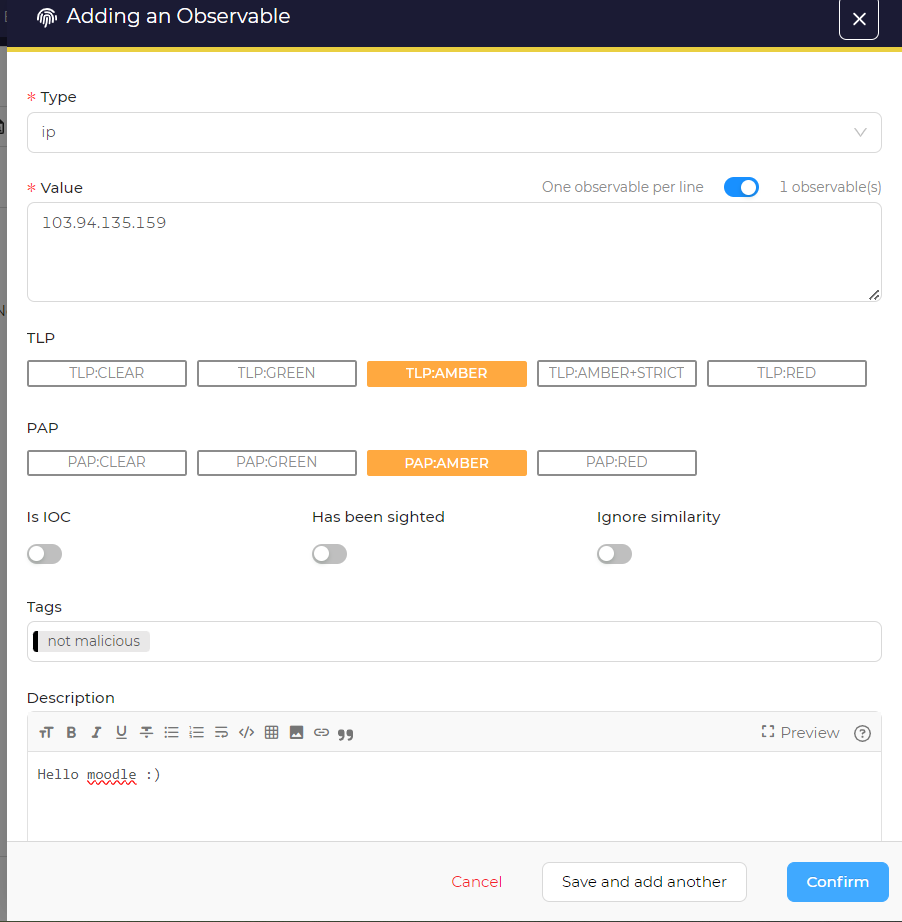
\includegraphics[width=233.9986pt,height=239.1871pt]{latexImage_0547928a85b55277de50b55b92e183c5.png}}
\put(221.649,-671.276){\fontsize{9.9626}{1}\usefont{T1}{cmr}{m}{n}\selectfont\color{color_29791}Figure 22: Creating observables}
\put(57,-696.836){\fontsize{9.9626}{1}\usefont{T1}{cmr}{m}{n}\selectfont\color{color_29791}Finally , click on Create Observable(s)}
\end{picture}
\begin{tikzpicture}[overlay]
\path(0pt,0pt);
\draw[color_29791,line width=0.996pt]
(57pt, -727.435pt) -- (525pt, -727.435pt)
;
\end{tikzpicture}
\begin{picture}(-5,0)(2.5,0)
\put(514.041,-739.888){\fontsize{9.9626}{1}\usefont{T1}{cmr}{b}{n}\selectfont\color{color_29791}27}
\end{picture}
\newpage
\begin{picture}(-5,0)(2.5,0)
\put(57,-71.96301){\fontsize{14.3462}{1}\usefont{T1}{cmr}{b}{n}\selectfont\color{color_29791}References}
\put(57,-93.784){\fontsize{9.9626}{1}\usefont{T1}{cmr}{m}{n}\selectfont\color{color_29791}[1]}
\put(67.51652,-93.784){\fontsize{9.9626}{1}\usefont{T1}{cmr}{m}{n}\selectfont\color{color_29791}}
\put(72.49782,-93.784){\fontsize{9.9626}{1}\usefont{T1}{cmr}{m}{n}\selectfont\color{color_29791}TheHive Project GitHub repository: https://github.com/TheHive- Project/TheHive}
\put(57,-111.716){\fontsize{9.9626}{1}\usefont{T1}{cmr}{m}{n}\selectfont\color{color_29791}[2]}
\put(67.51652,-111.716){\fontsize{9.9626}{1}\usefont{T1}{cmr}{m}{n}\selectfont\color{color_29791}}
\put(72.49782,-111.716){\fontsize{9.9626}{1}\usefont{T1}{cmr}{m}{n}\selectfont\color{color_29791}TheHive Project documentation: https://docs.thehive- project.org/thehive/}
\put(57,-129.649){\fontsize{9.9626}{1}\usefont{T1}{cmr}{m}{n}\selectfont\color{color_29791}[3]}
\put(67.51652,-129.649){\fontsize{9.9626}{1}\usefont{T1}{cmr}{m}{n}\selectfont\color{color_29791}}
\put(72.49782,-129.649){\fontsize{9.9626}{1}\usefont{T1}{cmr}{m}{n}\selectfont\color{color_29791}The hive ofiicial guide: https://docs.strangebee.com/thehive/setup/}
\end{picture}
\begin{tikzpicture}[overlay]
\path(0pt,0pt);
\draw[color_29791,line width=0.996pt]
(57pt, -727.435pt) -- (525pt, -727.435pt)
;
\end{tikzpicture}
\begin{picture}(-5,0)(2.5,0)
\put(514.041,-739.888){\fontsize{9.9626}{1}\usefont{T1}{cmr}{b}{n}\selectfont\color{color_29791}28}
\end{picture}
\end{document}